\documentclass[11pt]{article}
% ── ACL Standard Packages ─────────────────────────────────────
\usepackage[review]{acl}   % review = double-blind + line numbers
\usepackage{times}
\usepackage{latexsym}
\usepackage[T1]{fontenc}
\usepackage[utf8]{inputenc}
\usepackage{microtype}
\usepackage{inconsolata}
\usepackage{graphicx}
\usepackage{adjustbox}
% ── Original Paper Packages ───────────────────────────────────
\usepackage{amsmath,amssymb,amsfonts}
\usepackage{booktabs}
\usepackage{xcolor}
\usepackage{multirow}
\usepackage{array}
\usepackage{float}
\usepackage{placeins}
\usepackage{enumitem}
\usepackage{xurl}
\graphicspath{{figures/}{../output/figures/}{../output/mitigations/figures/}}
% ── Custom commands ───────────────────────────────────────────
\newcommand{\ie}{i.e.,\ }
\newcommand{\eg}{e.g.,\ }
\newcommand{\cf}{cf.\ }
\newcommand{\etal}{et~al.}
\newcommand{\wrt}{w.r.t.\ }
\newcommand{\pval}[1]{$p #1$}
% ── Title ─────────────────────────────────────────────────────
\title{No One Gets an A: Distributional Bias in LLM Text Scoring}
% Authors omitted for double-blind review.
\begin{document}
\maketitle
% ══════════════════════════════════════════════════════════════
% ABSTRACT
% ══════════════════════════════════════════════════════════════
\begin{abstract}
LLMs asked to rate text quality systematically avoid extreme scores,
compressing responses into a narrow interior band regardless of true
quality variation. We measure this \emph{score compression} across
eleven models (3.8B--228B parameters) via $\sim$99{,}000 evaluations
of 150 expert-authored articles, each degraded along four quality axes
(grammar, coherence, information, lexical sophistication) at five
controlled intensity levels. Compression ratios range from 0.026
(Mistral~7B) to 0.685 (GPT-5~mini), with a positive
size--compression correlation among nine open-weight models (Pearson
$r = 0.78$, $p = 0.013$). Neither GPT-5~mini nor Gemini~3~Flash ever
assigns 0 or 10 across 9{,}000 samples each---a pattern shared by
four additional models---despite simulations predicting hundreds of
such scores. A three-way mixed-effects model confirms significant main
effects and all interactions. Among five mitigation strategies on a
nine-model comparison, auxiliary regression yields the largest
pairwise-accuracy gain ($0.518 \to 0.702$), expected-score rescaling
improves rank correlation ($\rho\colon 0.458 \to 0.490$), and
quantile normalization recovers the full scale while preserving rank
order; contrastive anchor prompting produces mixed results. Post-hoc
affine calibration reduces RMSE by 10--26\%, confirming a systematic,
partially correctable distortion. These results demonstrate a robust
distributional bias in LLM-based text evaluation with direct
implications for any application relying on LLM-generated quality
ratings.
\end{abstract}
% ══════════════════════════════════════════════════════════════
% 1. INTRODUCTION
% ══════════════════════════════════════════════════════════════
\section{Introduction}
\label{sec:intro}

LLMs are increasingly deployed as automated text
evaluators---grading essays, rating content quality, scoring
summaries, and benchmarking generated text~\citep{zheng2023judging,liu2023geval,kocmi2023large}---under
the implicit assumption that they map quality onto numeric scales with
reasonable fidelity~\citep{zheng2023judging,liu2023geval}.

Yet LLMs exhibit a systematic reluctance to use
rating extremes~\citep{zheng2023judging,liu2023geval}: a pristine, publication-quality text consistently
receives 7 or 8 rather than 9 or 10, while heavily corrupted text
rarely drops below 2 or 3 (Table~\ref{tab:dist}; Figure~\ref{fig:histograms}).

This \emph{score compression} has significant practical consequences.
Compressing the effective range from $[0, 10]$ to roughly $[2, 9]$
reduces discriminative resolution by 30\% or more~\citep{zheng2023judging,liu2023geval},
degrades ranking reliability (Spearman $\rho$ as low as 0.138;
Table~\ref{tab:compression}), and miscalibrates threshold-based
decisions (\eg ``pass if score $\geq 7$''; Section~\ref{sec:calibration}).

Under a naive linear model, a text degraded to fraction $\lambda$ of
its original quality should score $S = 10(1 - \lambda)$. Instead, we
observe $S \approx 8 - 6.5\lambda$ for GPT-5~mini and $S \approx 8 -
6.2\lambda$ for Gemini~3~Flash (Section~\ref{sec:results},
Figure~\ref{fig:calibration})---the intercept falls short of 10 and
the slope reaches only $\sim$65\% of the ideal gradient
(Appendix~Table~\ref{tab:slopes_app}), compressing the usable range
by roughly a third.

The phenomenon we document---systematic under-utilisation of numeric
rating scales---constitutes a distinct class of evaluation failure we
term \emph{Distributional Bias}. Prior work has catalogued
\emph{selection} and \emph{categorical} biases in LLM judges,
including position bias~\citep{zheng2023judging,shi2024judging} and verbosity
bias~\citep{zheng2023judging}. These biases explain \emph{which} item a
model prefers~\citep{wang2024large}. Distributional bias, by contrast, describes a
structural failure in \emph{how} the model utilises the quantitative
scale to express that preference---regardless of which item is being
evaluated---a dimension absent from existing bias
taxonomies~\citep{zheng2023judging,wang2024large,liu2023geval}.

\citet{zheng2023judging} note scale-use tendencies but do not quantify
them; \citet{liu2023geval} observe miscalibration and propose a partial
remedy without systematic cross-model replication; \citet{wang2024large}
document ranking distortions but do not measure compression magnitude.
No prior work has \emph{quantified} compression magnitude against an algebraically
defined quality gradient, replicated it systematically across eleven
models spanning multiple providers and scales, or evaluated mitigation
strategies under controlled conditions. Our work provides this missing
quantitative foundation.

Whether distributional bias arises from RLHF training
dynamics~\citep{rafailov2023direct}, the mode-seeking property of
reverse KL-divergence~\citep{rafailov2023direct}, or token-frequency
effects in the pretraining corpus remains an open mechanistic question,
but the phenomenon itself is empirically tractable and consistently
reproduced across eleven diverse models
(Section~\ref{sec:multimodel}).

We present a controlled experiment to measure this precisely, with
three key features:
\begin{enumerate}[nosep]
    \item \textbf{Metamorphic behavioral testing~\citep{ribeiro2020beyond} with a known
    ground-truth gradient.} Metamorphic testing is a behavioral
    validation paradigm that probes model behavior through
    semantically meaningful input transformations with known expected
    output directions, without requiring ground-truth
    labels~\citep{ribeiro2020beyond}.
    Rather than comparing LLM judgments
    against noisy human annotations---which carry their own
    inter-rater disagreement and central-tendency
    biases~\citep{stevens1971issues}---we use deterministic,
    algorithmically defined degradations to construct a precisely
    controlled quality gradient~\citep{ribeiro2020beyond}. This
    guarantees that a Level~5 degradation is objectively worse than
    Level~1, providing a mathematical ground truth against which
    compression can be unambiguously measured
    (Section~\ref{sec:synthetic_justification}).
    \item \textbf{Psychometric axis isolation~\citep{attali2006automated,mcnamara2010linguistic}.}
    Psychometric axis isolation refers to the decomposition of writing
    quality into independent, theoretically grounded subscores---each
    targeting a distinct linguistic tier---so that degradation can be
    applied along one dimension at a time without confounding
    others~\citep{attali2006automated}. Following established
    Automated Essay Scoring (AES) frameworks~\citep{attali2006automated},
    degradation is applied along four independent axes---grammar,
    coherence, information content, and lexical sophistication---each
    targeting a distinct linguistic tier (surface syntax, discourse
    structure, semantics, and vocabulary)~\citep{mcnamara2010linguistic}.
    This isolates whether compression is uniform across quality
    dimensions or concentrated in specific cognitive tiers
    (Section~\ref{sec:axis_justification}).
    \item \textbf{Multi-model evaluation.} Eleven models spanning
    3.8B--228B parameters (Table~\ref{tab:models}), including frontier
    API models (GPT-5~mini, Gemini~3~Flash) and open-weight models
    from Meta, Google, Microsoft, Alibaba, Mistral~AI, and MiniMax,
    demonstrate that distributional bias is a robust cross-architecture
    phenomenon rather than a model-specific artifact
    (Section~\ref{sec:multimodel}).
\end{enumerate}
We declare three primary outcomes \emph{a priori}: (1) the compression
ratio per model (Section~\ref{sec:results}), (2) the average regression
slope of score on degradation level per model
(Section~\ref{sec:results}), and (3) the median paired score
difference between models on identical samples
(Section~\ref{sec:intermodel}).

Beyond documenting central tendency bias in a new
modality~\citep{stevens1971issues,guilford1954psychometric}, our
contributions are:
(i)~establishing \emph{distributional bias} as a
formally characterised taxonomy class, providing the first
\emph{quantified} compression magnitude against an algebraically
defined ground truth---whereas prior taxonomies either omit this
category or treat it as an incidental observation rather than a
primary failure mode~\citep{zheng2023judging,wang2024large};
(ii)~cross-model replication across eleven models spanning providers,
architectures, and scales (Table~\ref{tab:models});
(iii)~axis-specific sensitivity profiles revealing systematic
insensitivity to discourse-level
degradation~\citep{barzilay2008modeling,lapata2005automatic}
(Figure~\ref{fig:forest});
(iv)~a calibration recovery experiment showing a simple affine
transform reduces the gap by 10--26\% (Section~\ref{sec:calibration});
and
(v)~a systematic evaluation of five mitigation strategies showing
post-hoc corrections partially recover lost discriminative range
(Section~\ref{sec:mitigation}).

% ══════════════════════════════════════════════════════════════
% 2. RELATED WORK
% ══════════════════════════════════════════════════════════════
\section{Related Work}
\label{sec:related}

\subsection{LLM-as-a-Judge Bias Taxonomy}

Since the introduction of ``LLM-as-a-judge''
frameworks~\citep{zheng2023judging}, the NLP community has catalogued
a growing taxonomy of evaluation failure modes. Foundational work
identified primary categories: positional bias (favouring
candidates by order of appearance)~\citep{zheng2023judging,shi2024judging}
and verbosity bias (equating length with
quality)~\citep{zheng2023judging}.

\citet{wang2024large} further documented that quality rankings are
susceptible to positional bias, where the order of candidate responses
distorts evaluation outcomes, and established that LLM judges are
``unfair evaluators'' in a general sense.

\citet{li2025preference} introduced ``preference leakage,'' a
contamination problem in LLM-as-a-judge caused by the relatedness
between the synthetic data generator LLM and the judge LLM.

These early taxonomies focused primarily on \emph{selection} and
\emph{categorical} biases---explaining \emph{which} item a model
prefers~\citep{zheng2023judging,wang2024large,shi2024judging}. None of
these works \emph{quantify} compression magnitude against a controlled
ground truth or evaluate mitigation strategies systematically. Our
work fills this gap (Section~\ref{sec:mitigation}).

\subsection{Central Tendency Bias: Human Rating and LLM Outputs}

Human raters systematically avoid extremes on Likert scales,
compressing distributions around the
midpoint~\citep{stevens1971issues}; this is modulated by expertise,
scale length, and anchoring~\citep{guilford1954psychometric}.

AES models trained on human ratings inherit these
properties~\citep{ke2019automated}, and affine scaling methods to
recover lost variance are standard practice in traditional scoring
engines~\citep{attali2006automated}. However, those studies apply to
models \emph{fine-tuned} on human rating datasets~\citep{ke2019automated};
our study measures the intrinsic zero-shot calibration of
general-purpose instruct models---the setting describing the
overwhelming majority of LLM-as-judge deployments in
practice~\citep{zheng2023judging,liu2023geval}.

\subsection{Pointwise Scoring vs.\ Pairwise Ranking}

A growing body of evidence suggests that LLM judges excel at relative
pairwise comparison, whereas absolute point-wise scoring is
theoretically more unstable and prone to
fluctuation~\citep{zheng2023judging,liu2023geval}. Pointwise scoring
forces a broad distribution of potential human judgments into a single
deterministic label, causing models to default toward the centre of
the scale~\citep{liu2023geval,stevens1971issues}.

\citet{kocmi2023large} showed GPT-based metrics achieve
state-of-the-art MT correlation without examining distributional
properties; \citet{liu2023geval} found significant miscalibration and
proposed expected-score rescaling as a partial remedy
(Section~\ref{sec:mitigation}).

Our finding that models maintain high rank-order correlations
(Spearman $\rho$ up to 0.80) while simultaneously producing severe
absolute compression (CR as low as 0.026; Section~\ref{sec:results};
Table~\ref{tab:compression}) underscores why raw numeric scores must
be treated as ordinal rather than interval
signals~\citep{stevens1971issues}.

\subsection{RLHF and KL-Divergence as Compression Mechanisms}

A parallel mechanism for score compression operates at the level of
alignment training~\citep{rafailov2023direct}. In Reinforcement
Learning from Human Feedback (RLHF), the policy gradient objective
includes a KL divergence term that explicitly constrains the
fine-tuned policy $\pi_\theta$ to remain close to the reference
distribution $\pi_\text{ref}$~\citep{rafailov2023direct}:
\begin{equation}
    \mathcal{L}(\theta) = \mathbb{E}[r(x,y)] - \beta\,
    \text{KL}(\pi_\theta(y|x)\,\|\,\pi_\text{ref}(y|x))
    \label{eq:rlhf}
\end{equation}
This regulariser penalises high-variance outputs and discourages the
model from committing to extreme predictions that deviate from the
central mass of the training
distribution~\citep{rafailov2023direct}. Crucially, the reverse KL
divergence used in standard RLHF is mode-seeking: it concentrates
probability mass on the most likely outputs under the reference
policy, amplifying any existing central tendency in
$\pi_\text{ref}$~\citep{rafailov2023direct}. Because human preference
datasets themselves rarely contain extreme numeric
ratings~\citep{stevens1971issues}, the model learns to treat the
interior of the scale as the safe, aligned region.

\citet{rafailov2023direct} show that Direct Preference Optimization
(DPO) reparameterises this objective implicitly, but recent analysis
suggests DPO similarly contributes to distribution compression through
mode-seeking behaviour~\citep{rafailov2023direct}. This logit-level
effect compounds the distribution-level regularisation from RLHF,
jointly suppressing the probability mass assigned to extreme
outputs~\citep{rafailov2023direct}. Whether this training-time
mechanism is the primary driver of score compression remains an open
question; our experimental design documents the phenomenon rather than
isolating its cause (Section~\ref{sec:design}).

\subsection{Synthetic Perturbation Methodology}

To properly audit an LLM judge, we adopt a behavioral testing paradigm
grounded in the CheckList methodology~\citep{ribeiro2020beyond}, which
uses targeted Directional Expectation (DIR) perturbations---where
adding quality degradations \emph{should} reduce scores---rather than
held-out human labels to probe model behavior. The primary
justification over human baselines is the elimination of annotator
bias~\citep{stevens1971issues} and the provision of a mathematical
ground truth: a degradation at intensity $\lambda = 0.8$ is
objectively worse than $\lambda = 0.2$ by construction, independent
of any annotator's judgment~\citep{ribeiro2020beyond}.

% ══════════════════════════════════════════════════════════════
% 3. EXPERIMENTAL DESIGN
% ══════════════════════════════════════════════════════════════
\section{Experimental Design}
\label{sec:design}

\subsection{Rationale: Synthetic Perturbations vs.\ Human Baselines}
\label{sec:synthetic_justification}

Human judgment has historically served as the gold standard for NLP
evaluation, but modern meta-evaluation highlights its inherent
limitations: annotations are subject to inter-rater disagreement,
evaluator fatigue, and the evaluators' own central-tendency
biases~\citep{stevens1971issues}. More critically, accuracy-based
testing on human-annotated datasets may overestimate model performance
because both the model and the human labels may share statistical
shortcuts present in the training corpus~\citep{ribeiro2020beyond}.

To properly audit an LLM judge, we adopt a behavioral testing
paradigm grounded in the CheckList
methodology~\citep{ribeiro2020beyond}, which uses targeted
perturbations rather than held-out human labels to probe model
behavior. By employing deterministic, algorithmic perturbations, we
construct a precisely controlled quality gradient. This design
guarantees that a degradation at intensity level $\lambda = 0.8$ is
objectively worse than $\lambda = 0.2$ by construction, providing a
mathematical ground truth against which compression can be
definitively measured---independent of any human annotator's
judgment~\citep{ribeiro2020beyond}.

\subsection{The Four-Axis Quality Decomposition}
\label{sec:axis_justification}

The choice of four degradation axes is grounded in the psychometric
literature on text quality. Classic Automated Essay Scoring systems
such as the ETS e-rater decompose writing quality into subscores
covering surface mechanics, discourse coherence, content, and
vocabulary~\citep{attali2006automated}. Linguistic research confirms
that syntactic, discourse, semantic, and lexical features are
independent predictors of writing quality~\citep{mcnamara2010linguistic}.

By isolating surface syntax (Grammar), global discourse structure
(Coherence), factual completeness (Information), and vocabulary
richness (Lexical sophistication), we diagnose not only \emph{how
much} compression occurs, but \emph{which} linguistic dimensions LLM
evaluators weight most heavily. A uniform compression pattern across
all four axes would suggest a global numeric calibration failure;
axis-specific patterns would indicate qualitative blind spots in
evaluator sensitivity (Section~\ref{sec:results};
Figure~\ref{fig:forest}).

This axis decomposition is applied in a zero-shot, general-purpose
setting---in contrast to prior AES calibration work, which targets
models fine-tuned on human rating datasets~\citep{ke2019automated}.

\subsection{Corpus Construction}

The corpus comprises 150 articles from \emph{The Conversation}
(theconversation.com), where academic experts write evidence-based
articles for general audiences under professional editorial review.
Articles span five categories (Arts \& Culture, Business \& Economy,
Health, Politics \& Society, Science \& Technology) and are selected
at full length to ensure topical diversity.

\emph{The Conversation} was selected as corpus source because its
articles represent an unambiguous quality ceiling for the $\lambda =
0$ baseline: all content is produced by credentialed domain experts
and passes professional editorial review, eliminating the annotation
ambiguity present in crowdsourced or Wikipedia corpora. A corpus of
150 articles is consistent with practice in NLP evaluation metric
studies~\citep{kocmi2023large,liu2023geval}, where this sample size
provides sufficient statistical power for robustness assessment while
remaining feasible under API cost constraints.

\subsection{Degradation Engine}

Each article is degraded along exactly one of four orthogonal axes at
one of five levels $\lambda \in \{0.0, 0.2, 0.4, 0.6, 0.8\}$:
\begin{itemize}[nosep]
    \item \textbf{Grammar} ($G$): Surface-level mechanical errors
(typos, agreement violations, tense swaps, article errors,
homophones, preposition errors, word-order disruption) as
categorized by~\citet{attali2006automated}, implemented via
a nine-stage generation pipeline.
    \item \textbf{Coherence} ($C$): Bounded random sentence-order
    swaps, preserving all content and grammar. Random sentence
    shuffling is the standard benchmark for discourse coherence
    evaluation, disrupting local entity transitions and rhetorical
    structure while preserving sentence-level
    syntax~\citep{barzilay2008modeling,lapata2005automatic}.
    \item \textbf{Information} ($I$): Progressive content deletion via
    a five-phase pipeline targeting parentheticals, modifiers,
    prepositional phrases, subordinate clauses, and content
    words~\citep{attali2006automated}.
    \item \textbf{Lexical} ($L$): Vocabulary flattening by replacing
content words with high-frequency synonyms via word embedding
similarity, following established lexical simplification
methodology~\citep{glavas2015simplifying}.
\end{itemize}
At $\lambda = 0$, the original text is returned. The ceiling is
$\lambda = 0.8$ rather than $1.0$: full intensity on several axes
produces incoherent output that risks triggering model refusal rather
than scoring. All degradation functions are deterministic via
per-sample seeds:
$\text{MD5}(\text{title} \| \text{axis} \| \text{level} \|
\text{rep}) \bmod 2^{31}$.

\subsection{Factorial Design}

The experiment follows a $150 \times 4 \times 5 \times 3$ factorial
design:
\begin{equation}
    N = |\mathcal{C}| \times |\mathcal{A}| \times |\mathcal{L}| \times
    R = 150 \times 4 \times 5 \times 3 = 9{,}000
    \label{eq:design}
\end{equation}
The use of five stepped intensity levels follows standard practice in
synthetic perturbation studies~\citep{ribeiro2020beyond}, enabling
detection of both linear and non-linear sensitivity profiles across
the quality gradient. $R = 3$ repetitions per condition satisfies the
minimum requirement for reliable ICC(1,1) estimation
(Appendix~Table~\ref{tab:icc_app}) and allows characterisation of
intra-model scoring variance, yielding 9{,}000 samples per model and
99{,}000 total evaluations across all 11 models
(Table~\ref{tab:models}).

\subsection{Scoring Protocol}

Each sample is scored in isolation with the prompt: ``Rate the quality
of the following text from 0 to 10. Respond with ONLY the number.''
No rubric, examples, or reference texts are provided, measuring each
model's intrinsic calibration on an unanchored
scale~\citep{zheng2023judging}. This minimal prompt is intentional:
it targets zero-shot distributional bias as deployed in practice,
leaving the study of elaborate prompt designs (\eg chain-of-thought,
rubric-based scoring~\citep{liu2023geval}) to future work.

\begin{table}[htbp]
\centering
\caption{Models and configurations. All eleven models evaluated at
full factorial scale (9{,}000 samples each).}
\label{tab:models}
\begin{adjustbox}{max width=\columnwidth}
\begin{tabular}{@{}llrlll@{}}
\toprule
\textbf{Model} & \textbf{Provider} & \textbf{Params} & \textbf{Access}
& \textbf{Temp.} & \textbf{Logprobs} \\
\midrule
GPT-5 mini      & OpenAI         & ---  & API   & n/a & No  \\
Gemini 3 Flash  & Google         & ---  & API   & 0.0 & No  \\
GPT-OSS 120B    & Fireworks      & 120B & API   & 0.0 & Yes \\
MiniMax M2P1    & Fireworks      & 228B & API   & 0.0 & Yes \\
Gemma 2 9B      & Local (Ollama) & 9B   & Local & 0.0 & Yes \\
Llama 3.1 8B    & Local (Ollama) & 8B   & Local & 0.0 & Yes \\
Mistral 7B      & Local (Ollama) & 7B   & Local & 0.0 & Yes \\
Phi-4 14B       & Local (Ollama) & 14B  & Local & 0.0 & Yes \\
Phi-4 mini      & Local (Ollama) & 3.8B & Local & 0.0 & Yes \\
Qwen 2.5 14B    & Local (Ollama) & 14B  & Local & 0.0 & Yes \\
Qwen 2.5 7B     & Local (Ollama) & 7B   & Local & 0.0 & Yes \\
\bottomrule
\end{tabular}
\end{adjustbox}
\end{table}

GPT-5~mini is a reasoning model that does not support user-specified
temperature parameters. Passing \texttt{temperature} to the API
returns the error: \textit{``Unsupported parameter: `temperature' is
not supported with this model.''} The model's sampling behaviour is
therefore fixed at its internal default.\footnote{Empirically,
majority-vote aggregation over three repetitions yields near-identical
mean scores (mean absolute deviation from single-sample mean $<
0.05$), confirming that stochasticity does not materially affect our
results (Appendix~Table~\ref{tab:icc_app}).} Gemini~3~Flash runs at
temperature 0.0. The nine remaining models use temperature 0.0 and
return token-level log-probabilities, enabling logprob-based
mitigations (Section~\ref{sec:mitigation}).

% ══════════════════════════════════════════════════════════════
% 4. RESULTS
% ══════════════════════════════════════════════════════════════
\section{Results}
\label{sec:results}

Results are organized around the three primary outcomes, followed by
secondary analyses. All tables order models by descending compression
ratio.

\subsection{Score Distributions and Boundary Avoidance}

Most models use only a narrow subset of the 0--10 scale
(Table~\ref{tab:dist}). GPT-5~mini ($[1, 9]$), Gemini~3~Flash ($[2,
9]$), Gemma~2~9B, Llama~3.1~8B, Phi-4~14B, and Qwen~2.5~14B never
assign 0 or 10 across 9{,}000 samples each. Among the five models
that do produce extreme scores, MiniMax~M2P1 assigns 686 tens (7.7\%)
and GPT-OSS~120B assigns 394 zeros (4.4\%), while Mistral~7B,
Phi-4~mini, and Qwen~2.5~7B each produce fewer than 25 extreme
scores (Table~\ref{tab:dist}). Score means range from 4.23
(GPT-OSS~120B) to 8.62 (Qwen~2.5~7B), with smaller models clustering
at higher means and lower standard deviations, consistent with more
severe compression (Table~\ref{tab:dist};
Section~\ref{sec:multimodel}). Figure~\ref{fig:histograms} visualizes
all eleven distributions.

To test whether absent extreme scores merely reflect the experimental
design, we fit a linear model per model, simulate 100 datasets with
Gaussian noise at the observed residual SD, and count predicted
boundary scores. For the six models that never assign 0 or 10,
simulations predict substantial counts: GPT-5~mini should produce
$\sim$542 zeros and $\sim$122 tens; Gemini~3~Flash should produce
$\sim$73 zeros and $\sim$147 tens (Table~\ref{tab:dist}). The four
other boundary-free models show the same pattern. Among models that
do produce extreme scores, observed counts remain far below
predictions (\eg Mistral: 5 tens vs.\ $\sim$407 predicted),
confirming active boundary avoidance across the model landscape
(Figure~\ref{fig:histograms}; Figure~\ref{fig:perlevel}).

\begin{figure}[htbp]
\centering
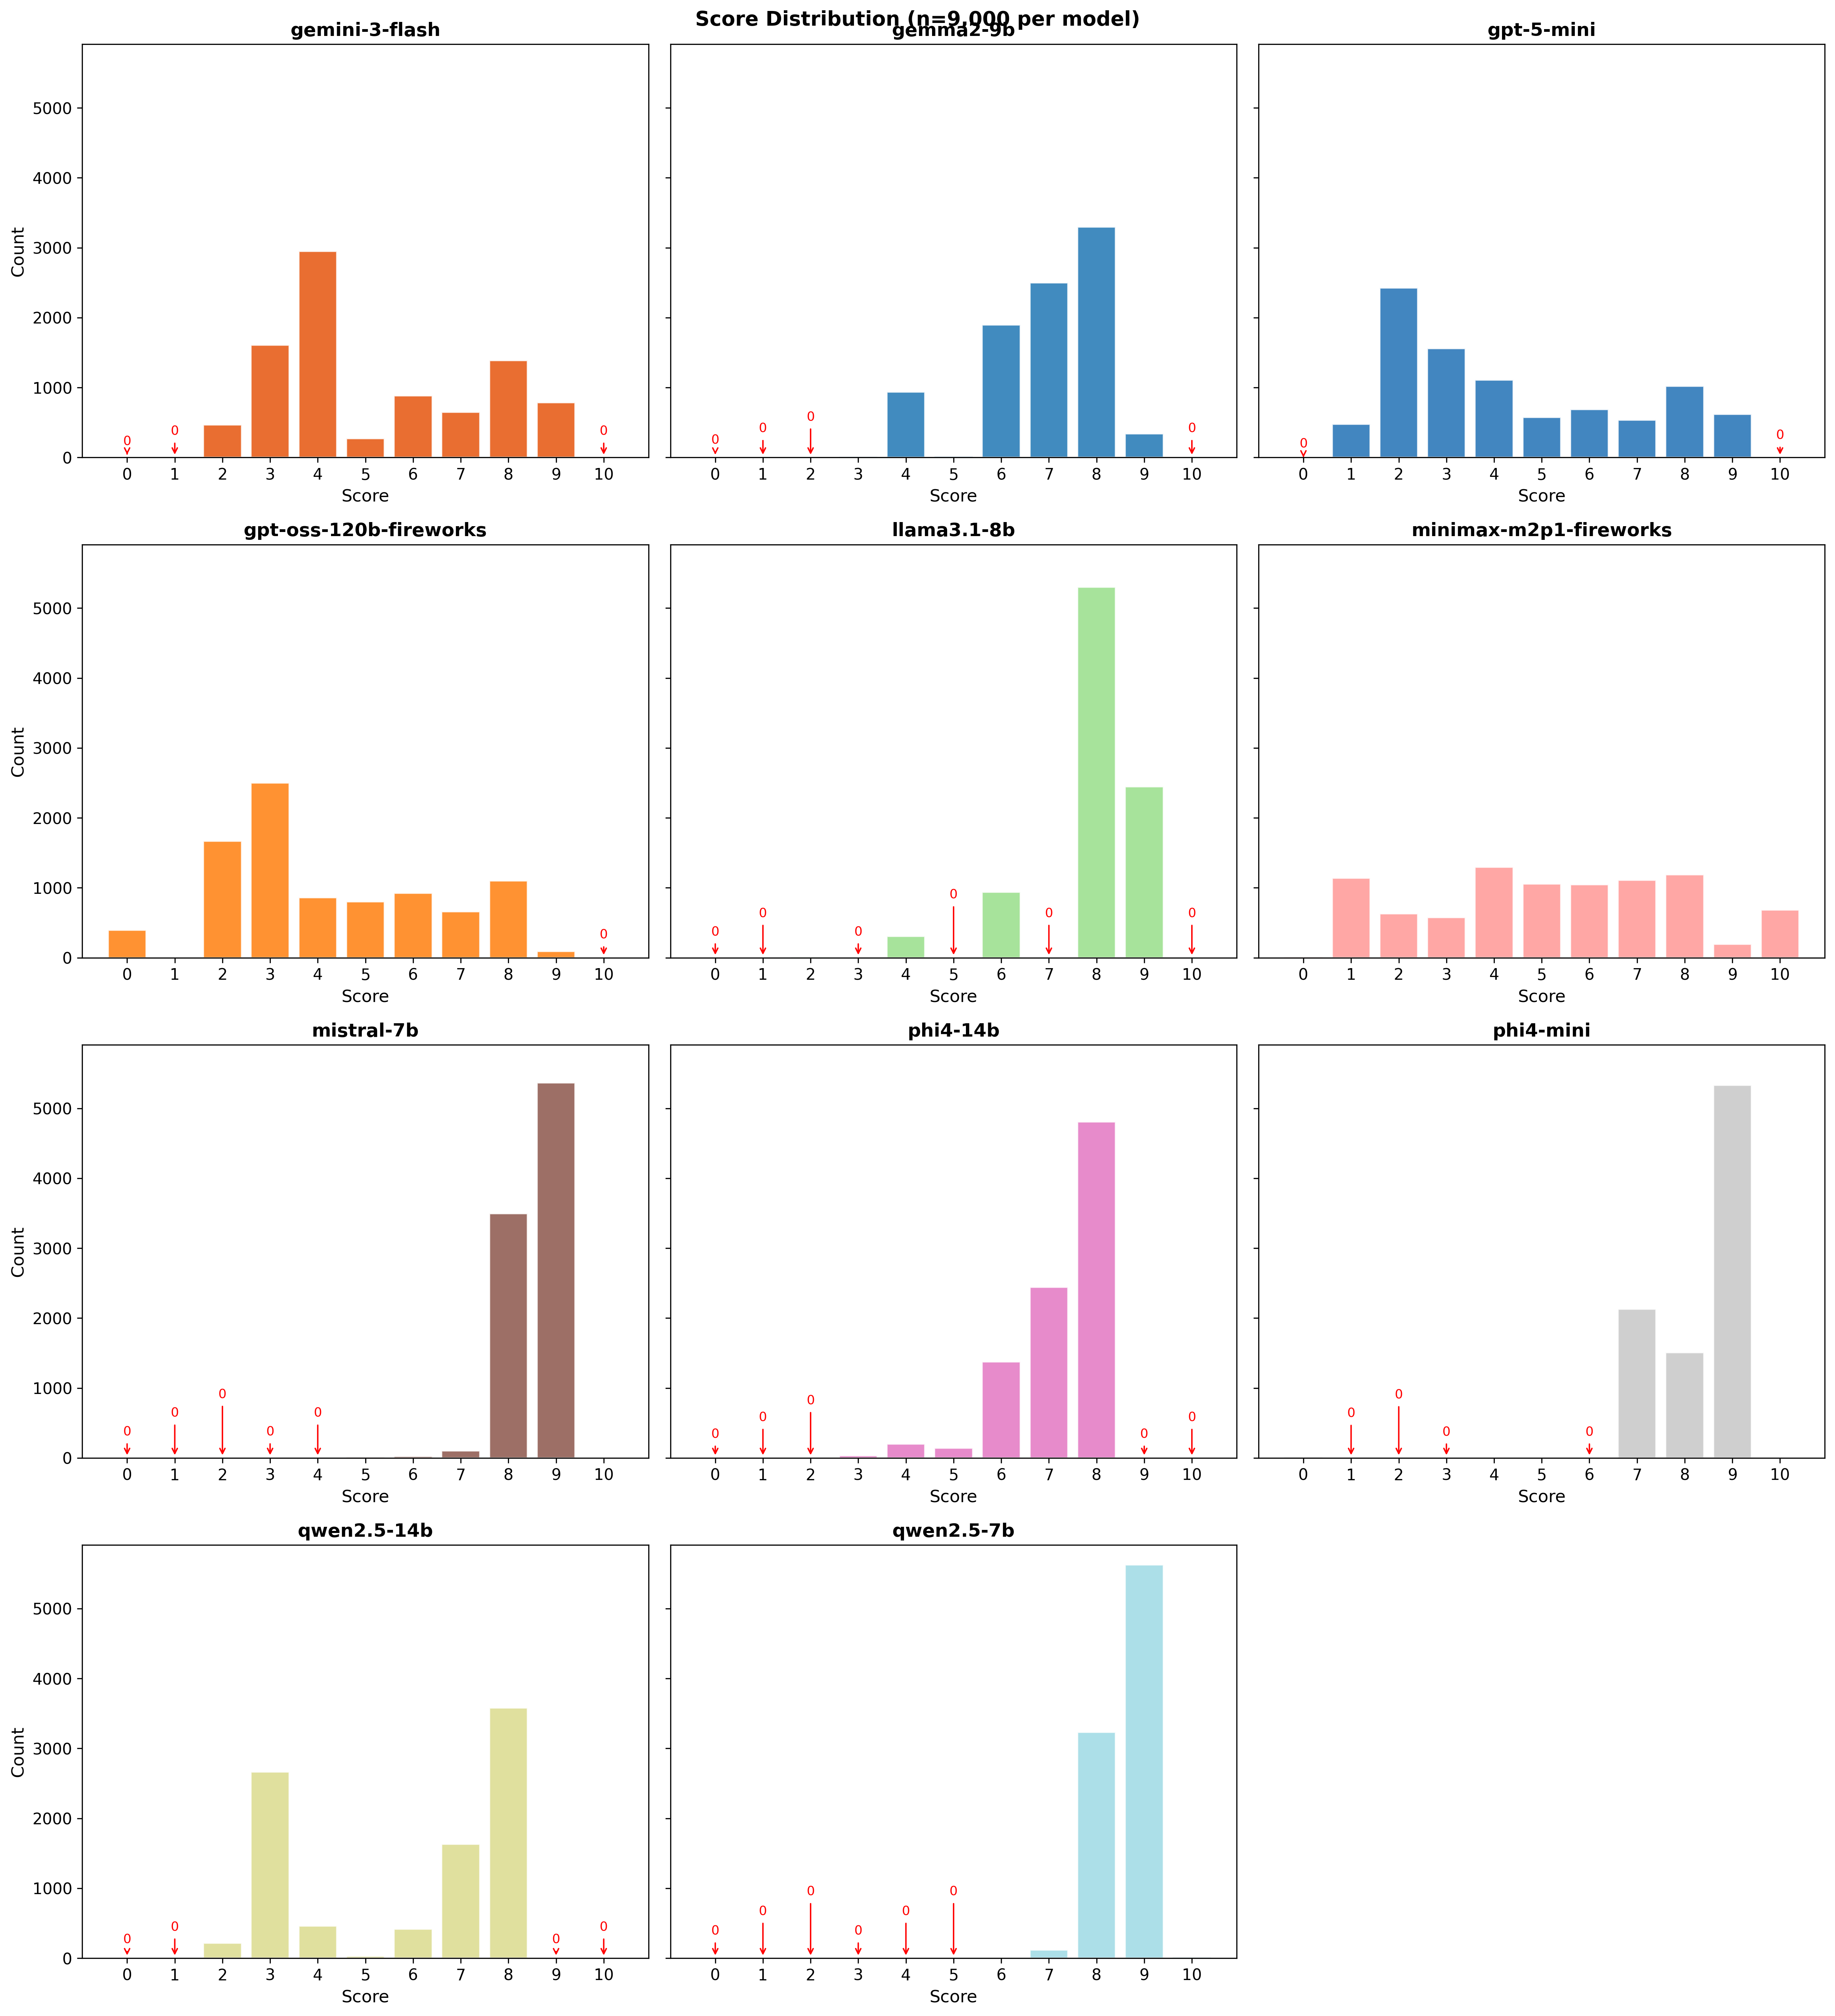
\includegraphics[width=\linewidth]{G3_score_histograms.png}
\caption{Score distributions for all eleven models ($n \approx
9{,}000$ per model). Red ``0'' annotations mark empty bins; bars
without annotation have small non-zero counts. Six models never assign
0 or 10; five produce rare or minority extreme scores
(Table~\ref{tab:dist}).}
\label{fig:histograms}
\end{figure}

\begin{table}[htbp]
\centering
\caption{Descriptive statistics ordered by compression ratio. Three
models returned $<$9{,}000 scores due to unparseable responses:
MiniMax~M2P1 ($n = 8{,}933$), Phi-4~mini ($n = 8{,}991$), Qwen~2.5~7B
($n = 8{,}998$).}
\label{tab:dist}
\small
\begin{adjustbox}{max width=\columnwidth}
\begin{tabular}{@{}lrccrccc@{}}
\toprule
\textbf{Model} & $n$ & \textbf{Mean} & \textbf{SD} & \textbf{Range} &
\textbf{Skew} & \textbf{\#0s} & \textbf{\#10s} \\
\midrule
GPT-5 mini      & 9{,}000 & 4.32 & 2.46 & 1--9  &  0.57  & 0   & 0   \\
Gemini 3 Flash  & 9{,}000 & 5.21 & 2.15 & 2--9  &  0.43  & 0   & 0   \\
GPT-OSS 120B    & 9{,}000 & 4.23 & 2.25 & 0--9  &  0.35  & 394 & 0   \\
Qwen 2.5 14B    & 9{,}000 & 5.89 & 2.24 & 2--8  & $-$0.43 & 0   & 0   \\
MiniMax M2P1    & 8{,}933 & 5.23 & 2.67 & 0--10 & $-$0.01 & 8   & 686 \\
Gemma 2 9B      & 9{,}000 & 6.91 & 1.30 & 3--9  & $-$0.91 & 0   & 0   \\
Phi-4 14B       & 9{,}000 & 7.27 & 0.97 & 3--8  & $-$1.49 & 0   & 0   \\
Llama 3.1 8B    & 9{,}000 & 7.92 & 1.12 & 2--9  & $-$1.85 & 0   & 0   \\
Phi-4 mini      & 8{,}991 & 8.34 & 0.91 & 0--10 & $-$1.88 & 15  & 3   \\
Qwen 2.5 7B     & 8{,}998 & 8.62 & 0.52 & 6--10 & $-$0.75 & 0   & 21  \\
Mistral 7B      & 9{,}000 & 8.58 & 0.55 & 5--10 & $-$1.05 & 0   & 5   \\
\bottomrule
\end{tabular}
\end{adjustbox}
\end{table}

\subsection{Primary Outcome 1: Compression Ratio}

Under a naive linear scorer mapping $\lambda$ to $S = 10(1 - \lambda)$,
the expected score span between $\lambda = 0$ and $\lambda = 0.8$ is
8 points. The compression ratio is:
\begin{equation}
    \mathit{CR} = \frac{\bar{S}(\lambda = 0) - \bar{S}(\lambda =
    0.8)}{10(1 - 0) - 10(1 - 0.8)} = \frac{\bar{S}(0) -
    \bar{S}(0.8)}{8}
    \label{eq:compression}
\end{equation}
$\mathit{CR} = 1$ indicates no compression; $\mathit{CR} < 1$
indicates compression.

\begin{table}[htbp]
\centering
\caption{Compression ratio (CR) with 95\% block-bootstrap CIs
(10{,}000 iterations) and Spearman $\rho$ for all eleven models. All
CIs exclude 1.0.}
\label{tab:compression}
\small
\begin{adjustbox}{max width=\columnwidth}
\begin{tabular}{@{}lrccc@{}}
\toprule
\textbf{Model} & \textbf{Params} & $\widehat{\mathit{CR}}$ &
\textbf{95\% CI} & \textbf{Spearman} $\rho$ \\
\midrule
GPT-5 mini      & ---  & 0.685 & [0.667, 0.700] & 0.729 \\
Gemini 3 Flash  & ---  & 0.620 & [0.603, 0.635] & 0.801 \\
GPT-OSS 120B    & 120B & 0.504 & [0.470, 0.537] & 0.617 \\
Qwen 2.5 14B    & 14B  & 0.446 & [0.431, 0.461] & 0.618 \\
MiniMax M2P1    & 228B & 0.420 & [0.392, 0.447] & 0.473 \\
Gemma 2 9B      & 9B   & 0.299 & [0.288, 0.311] & 0.704 \\
Phi-4 14B       & 14B  & 0.177 & [0.168, 0.187] & 0.548 \\
Llama 3.1 8B    & 8B   & 0.157 & [0.148, 0.166] & 0.464 \\
Phi-4 mini      & 3.8B & 0.078 & [0.067, 0.089] & 0.239 \\
Qwen 2.5 7B     & 7B   & 0.056 & [0.049, 0.064] & 0.324 \\
Mistral 7B      & 7B   & 0.026 & [0.018, 0.034] & 0.138 \\
\bottomrule
\end{tabular}
\end{adjustbox}
\end{table}

All eleven models compress below the ideal (Table~\ref{tab:compression}),
with CRs from 0.026 (Mistral~7B) to 0.685 (GPT-5~mini). All CIs
exclude 1.0, confirming statistical robustness. Sub-10B models all
achieve CR $< 0.30$; models above 100B all reach 0.42 or higher
(Table~\ref{tab:compression}; Section~\ref{sec:multimodel}).

Notably, CR and rank correlation are dissociated: Gemma~2~9B
achieves Spearman $\rho = 0.704$ despite a modest CR of 0.299
(Table~\ref{tab:compression}), indicating that models can preserve
relative quality ordering within a compressed absolute range. This
dissociation is consistent with evidence that LLMs function more
reliably as relative rankers than as absolute point-wise scorers,
which suffer from severe score concentration and a lack of
discriminative resolution~\citep{zheng2023judging,liu2023geval}.

Figure~\ref{fig:calibration} shows the compression gap against the
calibration reference.

\begin{figure}[htbp]
\centering
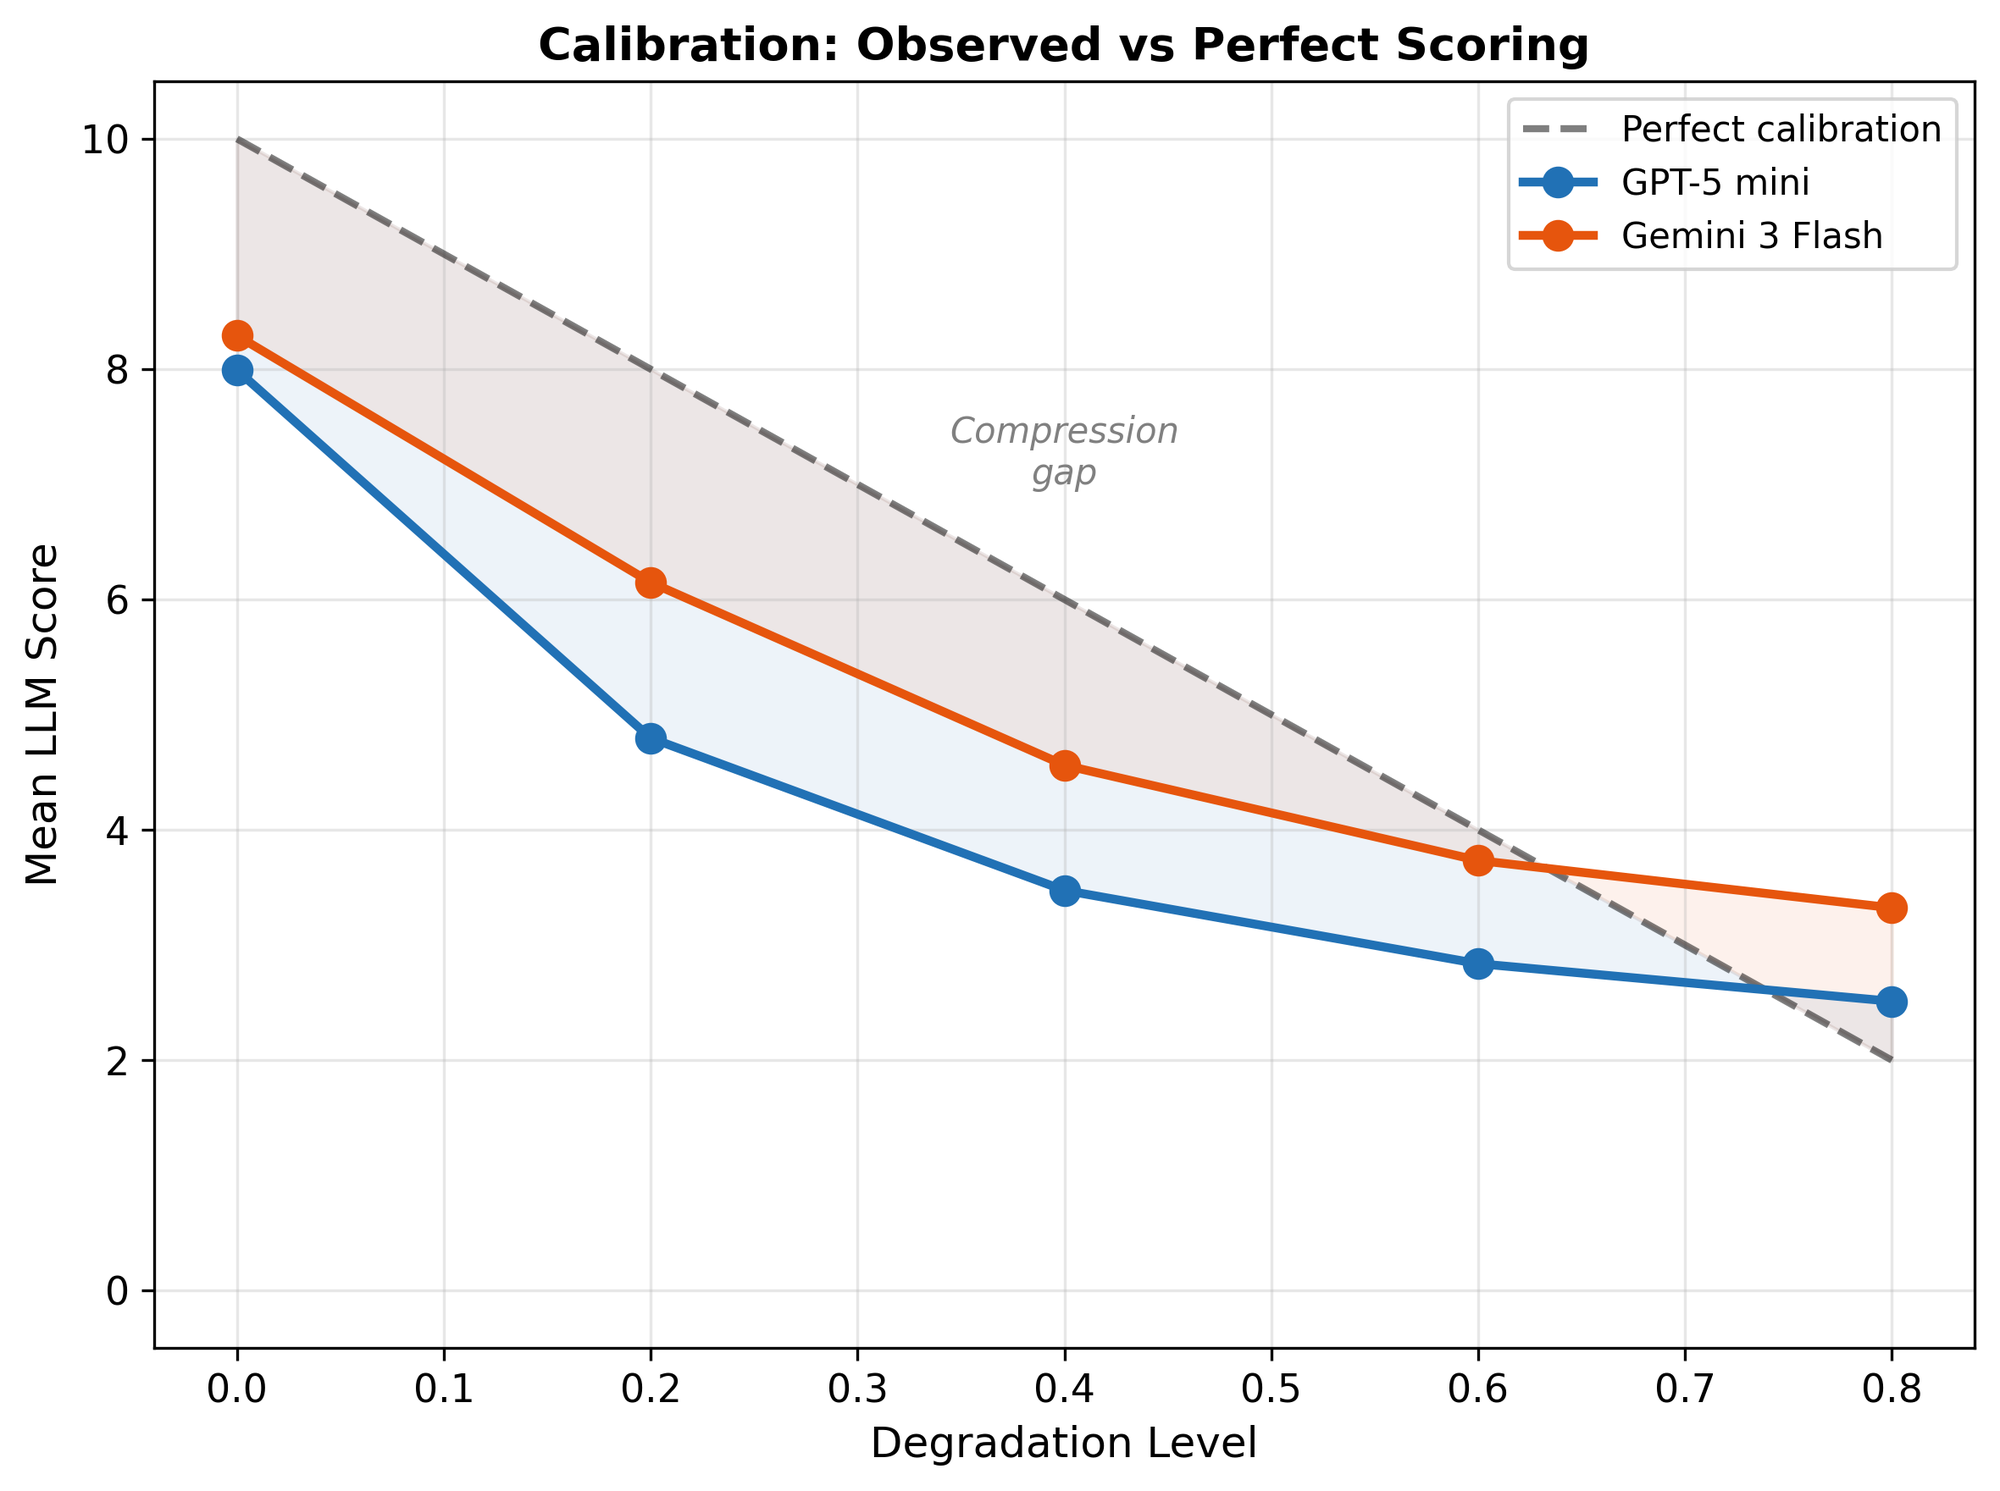
\includegraphics[width=\linewidth]{G9_calibration.png}
\caption{Calibration plot: observed mean scores vs.\ the naive
reference $S = 10(1 - \lambda)$. Shaded area represents the
compression gap.}
\label{fig:calibration}
\end{figure}

\subsection{Primary Outcome 2: Sensitivity (Regression Slopes)}

Linear regression of score on degradation level quantifies model
sensitivity (Figure~\ref{fig:forest}; full values in
Appendix~Table~\ref{tab:slopes_app}). Across all eleven models, 43 of
44 slopes are significantly negative ($p < 0.001$); the exception is
Mistral~7B on lexical degradation ($\beta_1 = -0.03$, $p = 0.49$;
Appendix~Table~\ref{tab:slopes_app}). Information deletion produces
the steepest slopes for both GPT-5~mini ($\beta_1 = -7.87$) and
Gemini~3~Flash ($-7.05$; Appendix~Table~\ref{tab:slopes_app});
coherence disruption is shallowest for GPT-5~mini ($-4.78$) and
lexical degradation shallowest for Gemini~3~Flash ($-5.26$). Mean
slopes range from $-6.46$ (GPT-5~mini) to $-0.28$ (Mistral~7B),
versus the ideal $-10$ (Appendix~Table~\ref{tab:slopes_app}). Only
the top API models reach two-thirds of ideal sensitivity; nine of
eleven models achieve less than half.

The consistently shallow coherence slopes are particularly noteworthy.
Random sentence shuffling destroys argumentative flow and entity-grid
coherence transitions~\citep{barzilay2008modeling} while preserving
all surface features, yet models penalise this disruption far less
than equivalent-intensity grammatical or informational degradation.
This suggests that point-wise LLM evaluation relies disproportionately
on local, sentence-level fluency signals over global discourse
structure~\citep{barzilay2008modeling,lapata2005automatic}.

\begin{figure}[htbp]
\centering
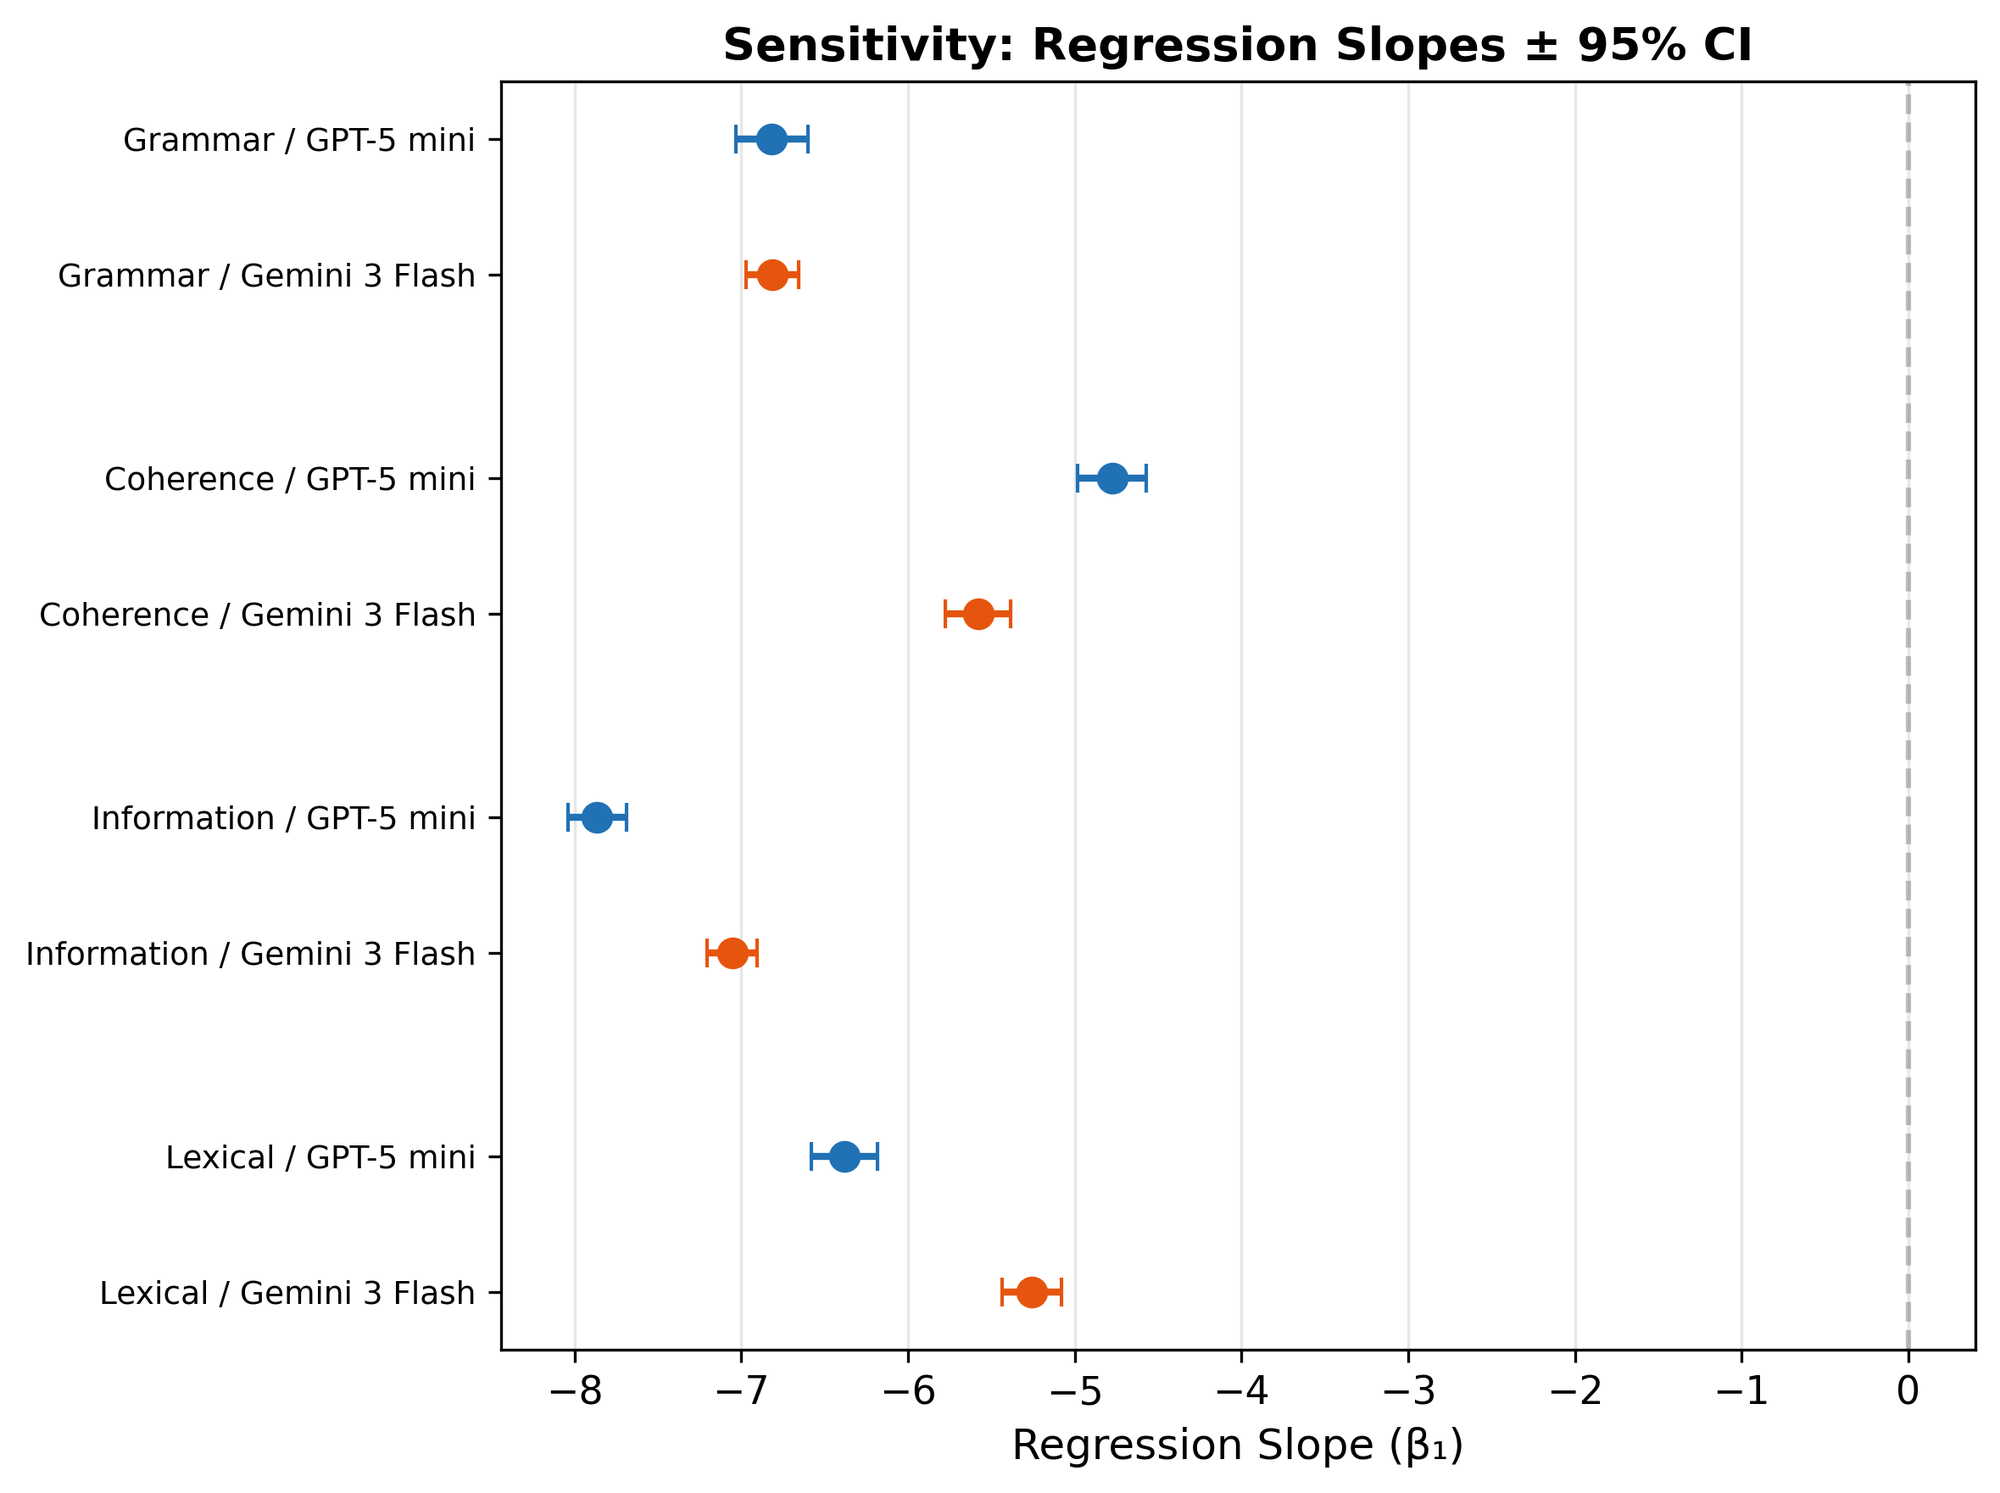
\includegraphics[width=\linewidth,height=0.65\textheight,keepaspectratio]{G8_forest_plot.png}
\caption{Forest plot of regression slopes ($\beta_1$) with 95\% CIs
across all axis$\times$model combinations. All slopes significantly
negative except Mistral~7B lexical.}
\label{fig:forest}
\end{figure}

\begin{figure}[htbp]
\centering
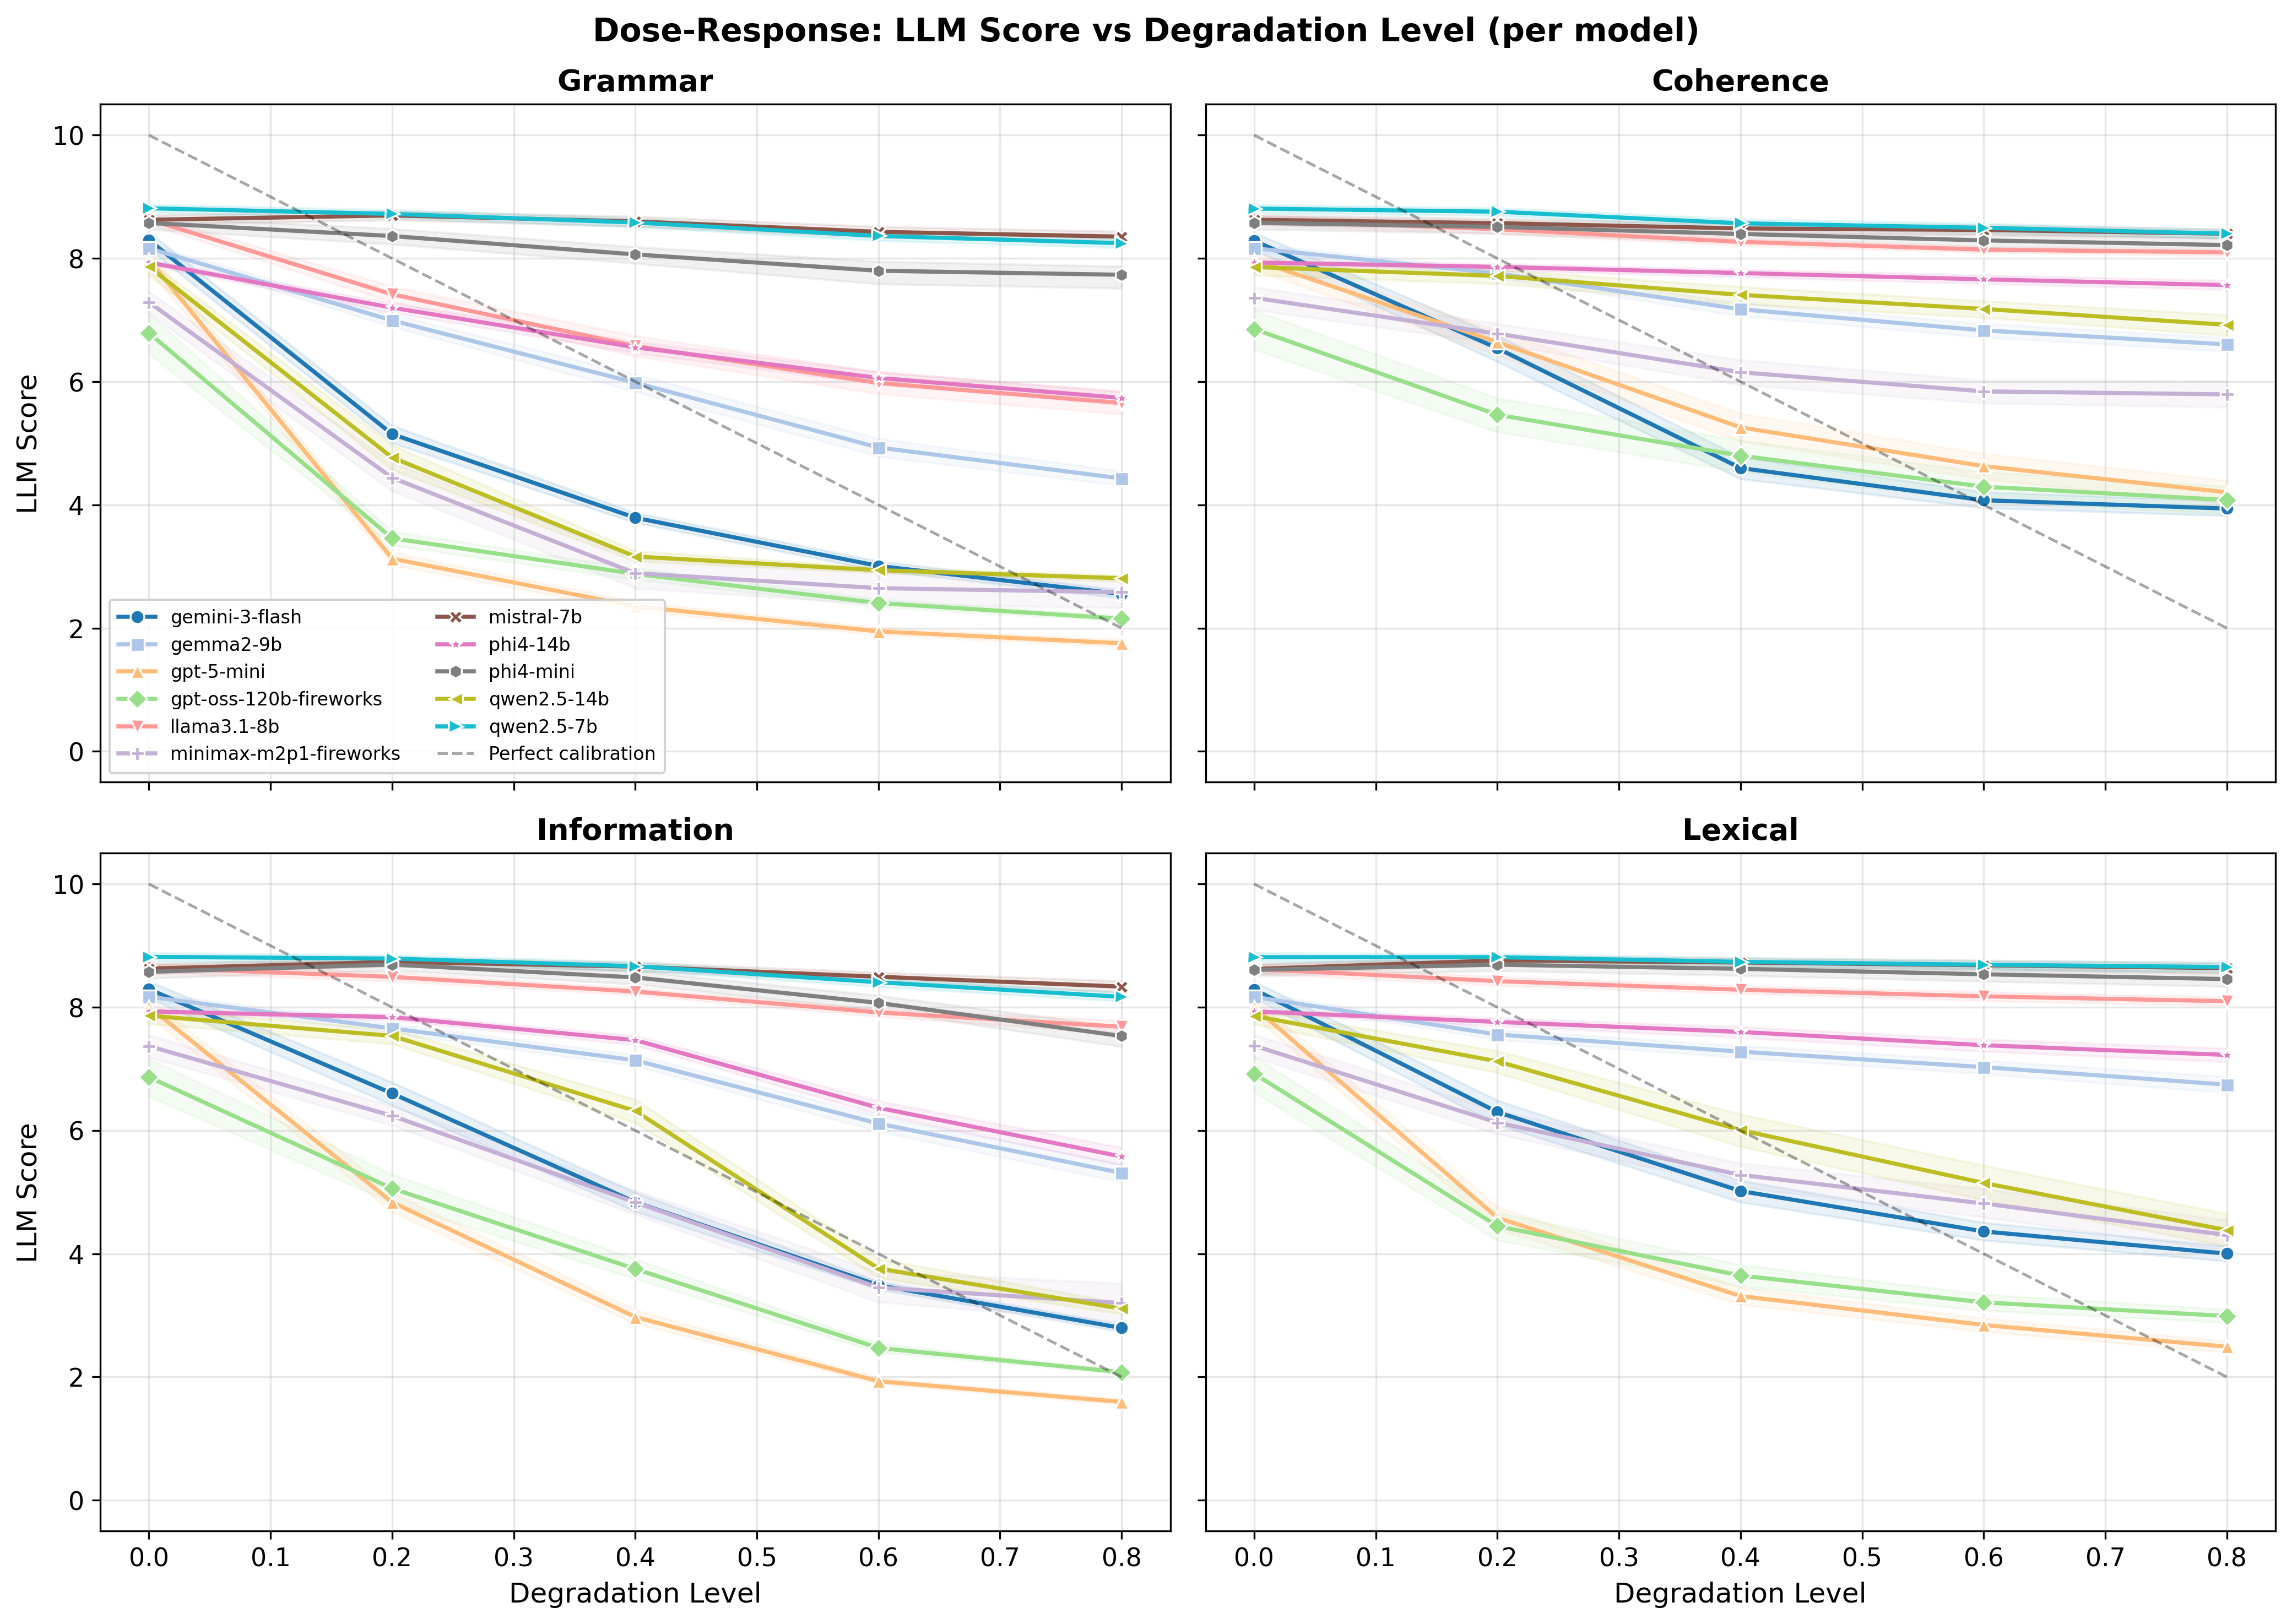
\includegraphics[width=\linewidth]{G1_dose_response.png}
\caption{Dose-response curves: mean score vs.\ degradation level per
axis. Shaded bands = 95\% block-bootstrap CIs (5{,}000 iterations).
Dashed line = naive linear reference. Concave shape reflects
diminishing sensitivity at higher degradation.}
\label{fig:doseresponse}
\end{figure}

\subsection{Secondary Diagnostics}
\label{sec:diagnostics}

Secondary diagnostics confirm that score--degradation relationships
are strictly monotonic but mildly concave, peaking in sensitivity at
low degradation (Figure~\ref{fig:doseresponse}). Score variance
exhibits a heteroscedastic ``fan-out-then-in'' pattern---peaking at
intermediate degradation levels (Figure~\ref{fig:boxplots};
Figure~\ref{fig:violins})---consistent with the hard ceiling and
floor compression effects described above. Detailed non-linearity
$F$-tests (Appendix~Table~\ref{tab:nonlin}), Kendall's $\tau$ rank
correlations (Appendix~Table~\ref{tab:tau}), and variance diagnostics
(Figure~\ref{fig:residuals}) are provided in
Appendix~\ref{app:diagnostics}.

\subsection{Mixed-Effects Model}
\label{sec:mixedeffects}

The next two subsections focus on GPT-5~mini and Gemini~3~Flash---the
two highest-performing frontier models---selected because they
represent distinct API providers and both achieve CR $> 0.60$ and
Spearman $\rho > 0.70$ (Table~\ref{tab:compression}). The three-way
specification requires exactly two model levels; inter-model agreement
metrics are inherently pairwise.

The model
\begin{equation}
    S_{ijk} \sim \lambda \times \mathrm{Axis} \times \mathrm{Model} +
    (1 + \lambda \mid \text{Article})
\end{equation}
converged with random intercepts and slopes. Key findings (full
coefficients in Appendix~Table~\ref{tab:mixedeffects_app}):
\begin{itemize}[nosep]
    \item Degradation level: large negative main effect ($\beta =
    -4.76$, $z = -45.6$, $p < 10^{-300}$).
    \item Model intercept (Gemini vs.\ GPT): non-significant ($\beta =
    +0.07$, $p = 0.25$), indicating comparable baseline scoring at
    $\lambda = 0$. The significant $+1$ point median offset
    (Section~\ref{sec:intermodel}) emerges from interaction terms as
    degradation increases.
    \item All axis main effects significant; grammar shows the largest
    intercept reduction ($\beta = -1.49$, $z = -25.1$).
    \item All three-way $\mathrm{Level} \times \mathrm{Axis} \times
    \mathrm{Model}$ interactions significant. Largest: $\mathrm{Level}
    \times \mathrm{Lexical} \times \mathrm{Gemini}$ ($\beta = +1.93$,
    $z = +11.2$), confirming Gemini is substantially less sensitive to
    lexical degradation (Appendix~Table~\ref{tab:slopes_app}).
    \item Random effects: article-level intercept variance $= 0.54$;
    slope variance $= 0.49$ (Appendix~Table~\ref{tab:mixedeffects_app}).
\end{itemize}

\subsection{Primary Outcome 3: Inter-Model Comparison}
\label{sec:intermodel}

Despite high agreement (Pearson $r = 0.836$, Spearman $\rho = 0.817$,
quadratic weighted $\kappa = 0.772$), Gemini~3~Flash scores
systematically higher than GPT-5~mini by a median of $+1$ point ($p <
10^{-300}$, rank-biserial $r = +0.705$). This offset is present
across all four axes: largest on grammar, information, and lexical
($+1$); smallest on coherence ($0$). All per-axis Wilcoxon tests are
significant after Benjamini-Hochberg correction
(Appendix~Table~\ref{tab:slopes_app}).

Figures~\ref{fig:scatter}--\ref{fig:paireddiff} show the agreement
scatter and paired-difference distribution.

\begin{figure}[htbp]
\centering
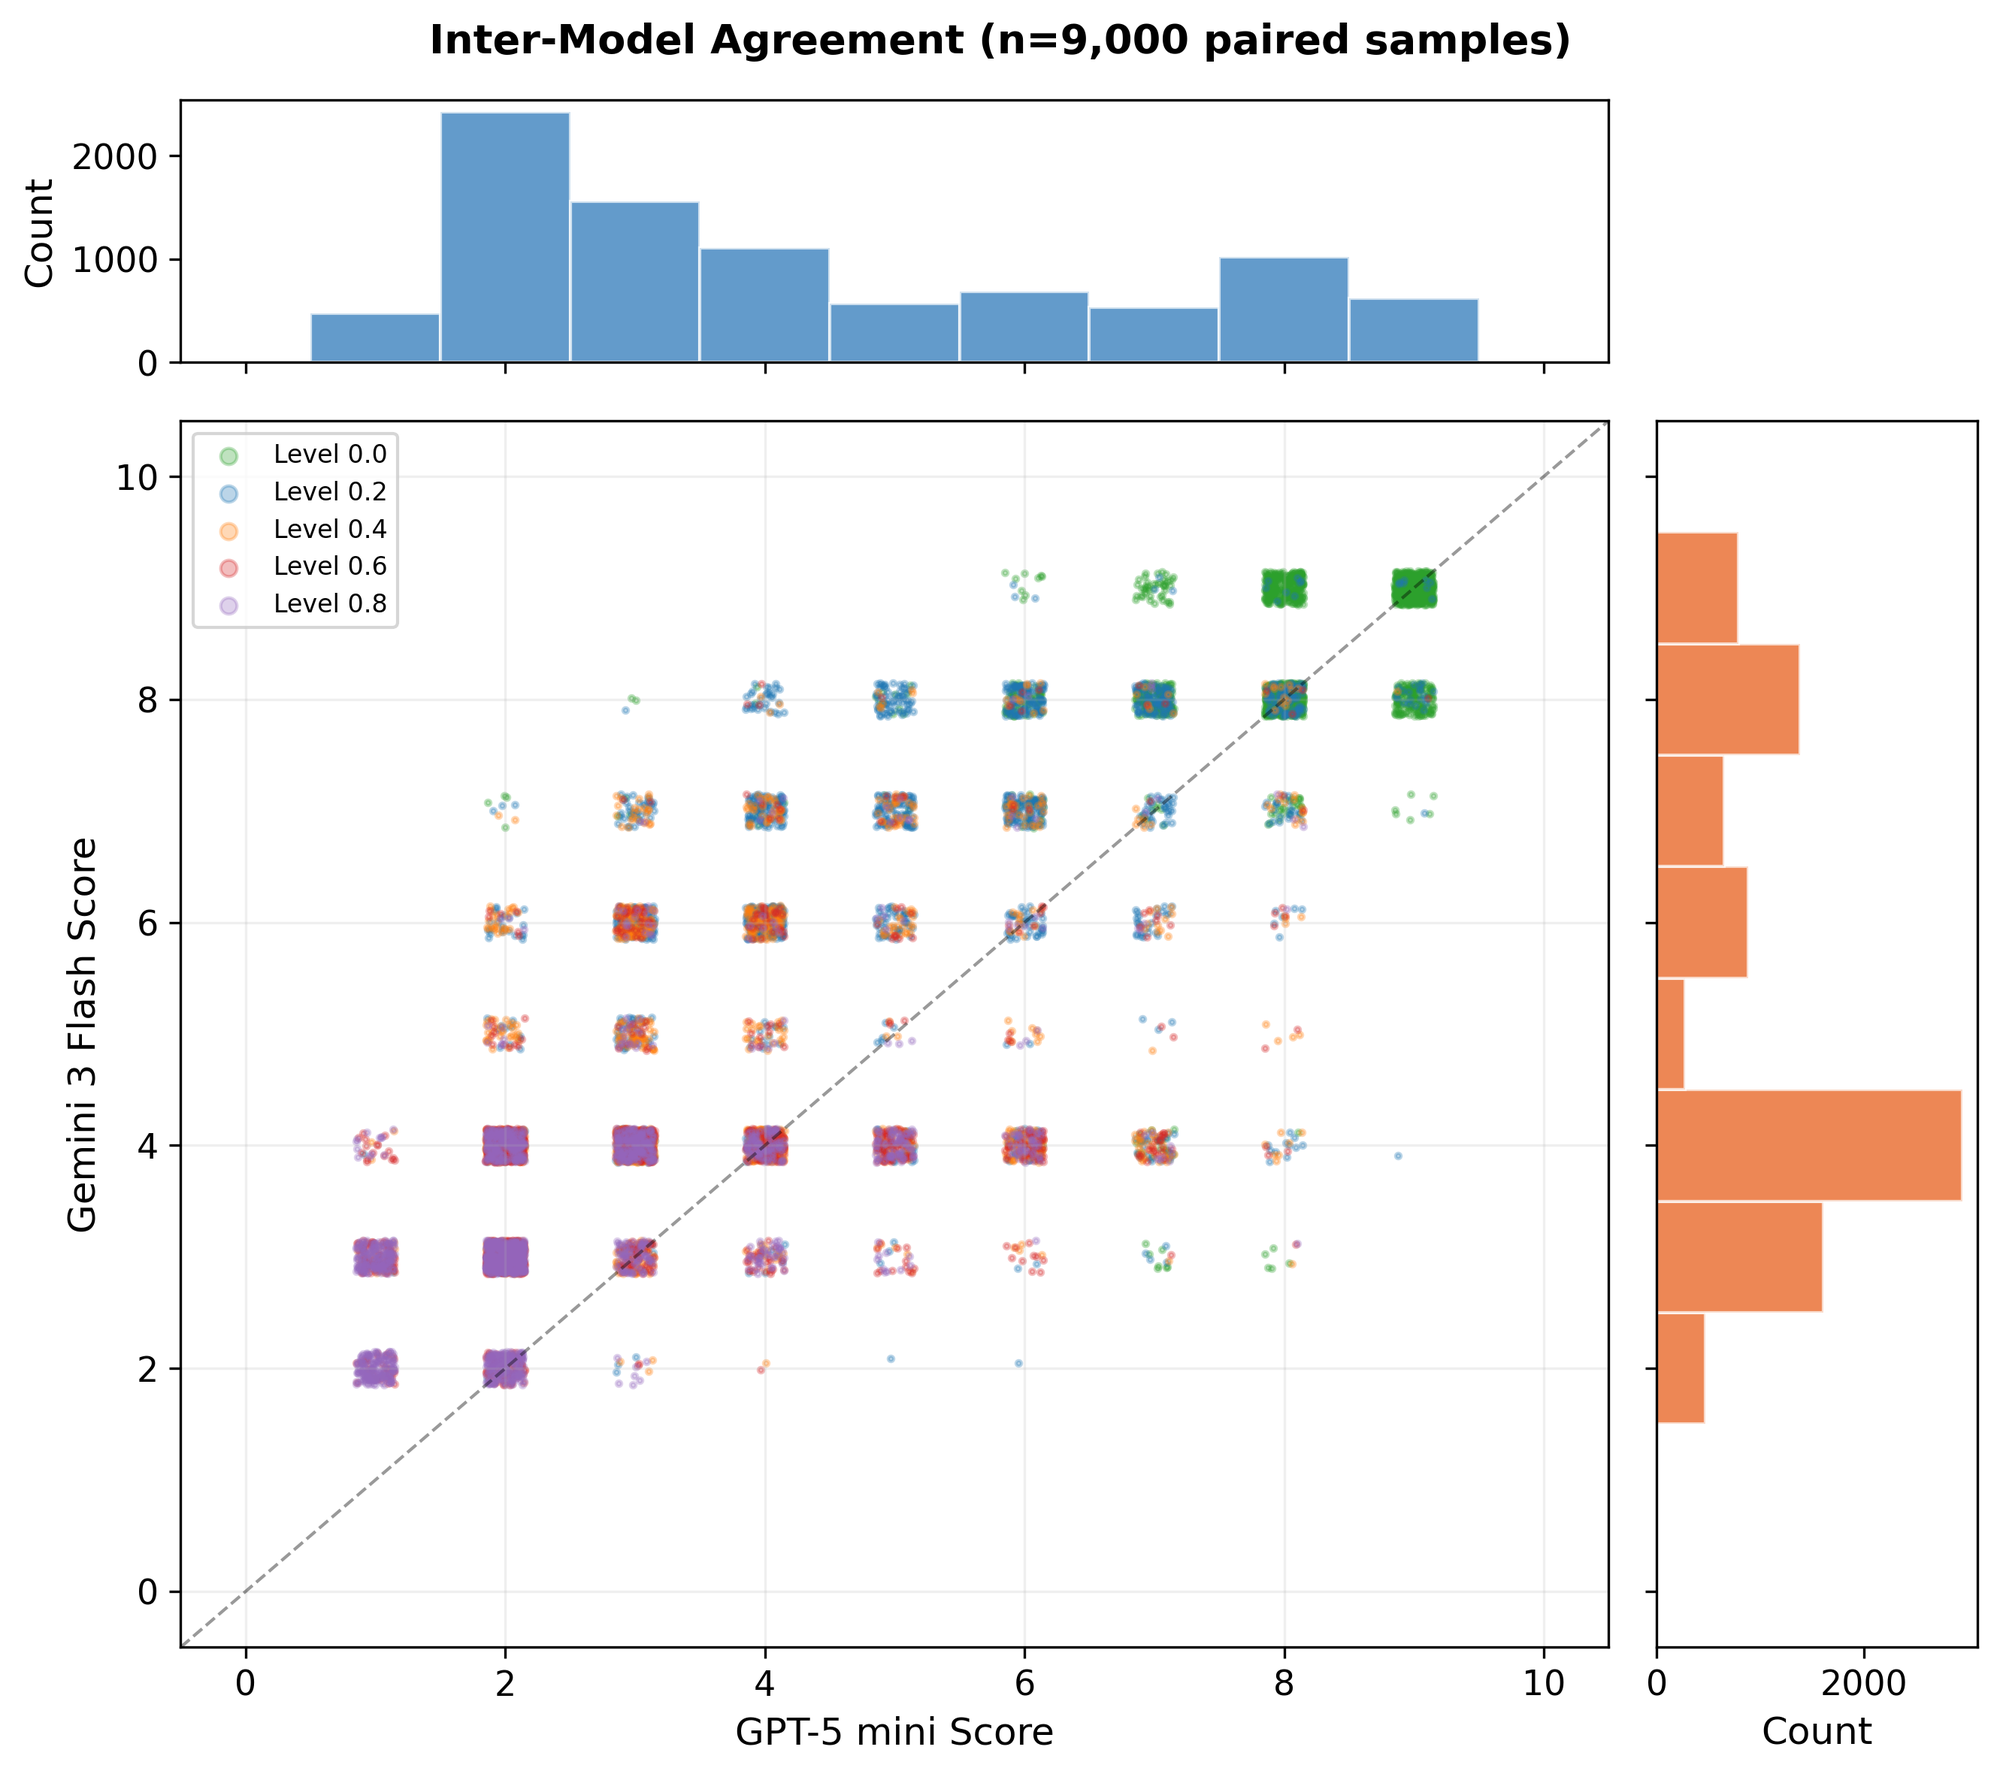
\includegraphics[width=\linewidth]{G10_inter_model_scatter.png}
\caption{Inter-model scatter ($n = 9{,}000$ paired samples), jittered
and colored by degradation level. Points above the identity line
indicate Gemini scored higher.}
\label{fig:scatter}
\end{figure}

\begin{figure}[htbp]
\centering
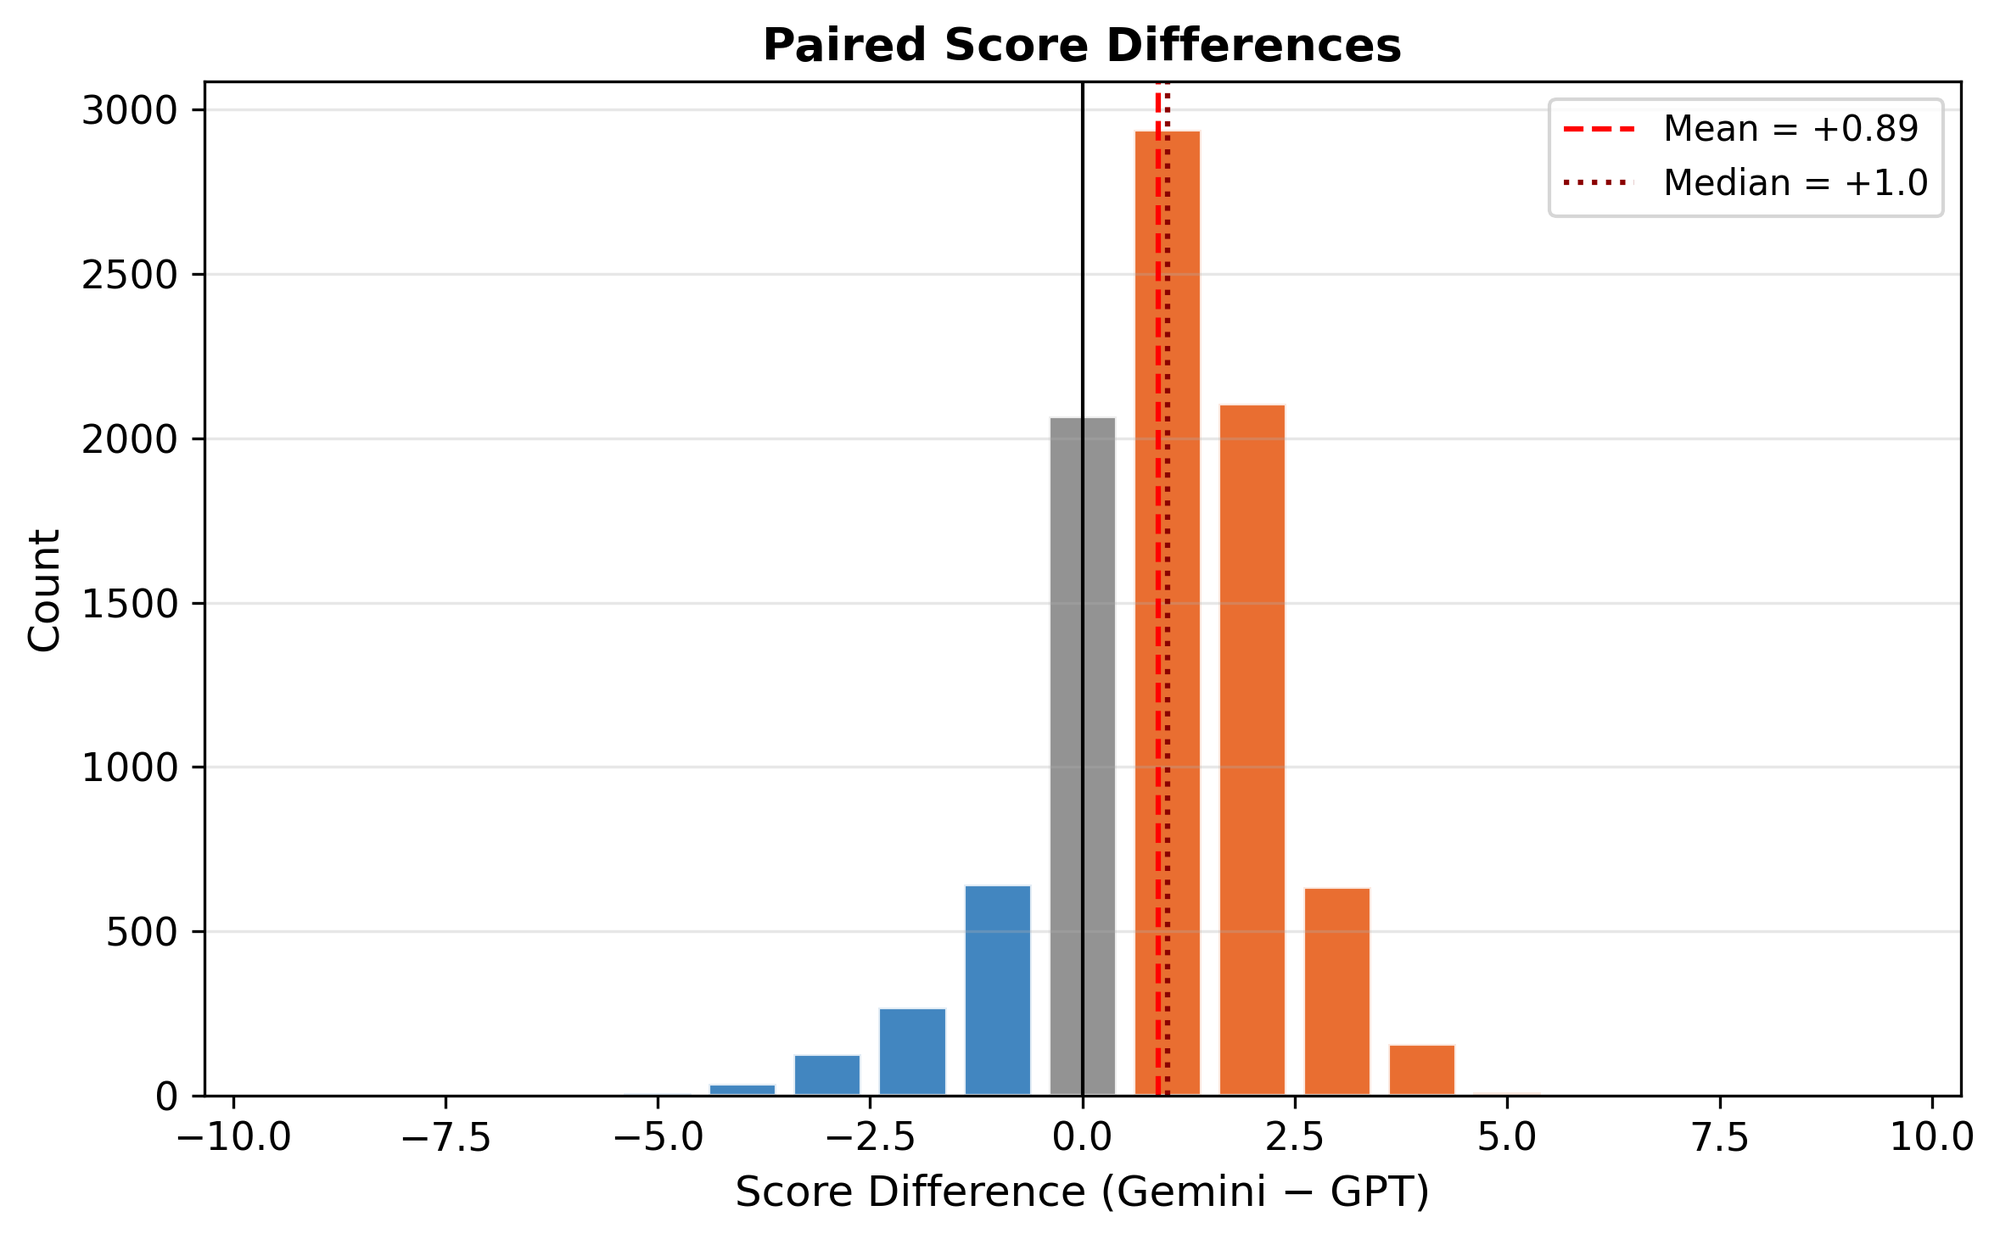
\includegraphics[width=\linewidth]{G11_paired_diff.png}
\caption{Paired score differences (Gemini $-$ GPT): right-shifted
distribution with median $+1$, mean $+0.89$.}
\label{fig:paireddiff}
\end{figure}

\subsection{Calibration Recovery}
\label{sec:calibration}

To test post-hoc correctability, we split 150 articles 80/20
(training: 120 articles, 7{,}200 samples; test: 30 articles, 1{,}800
samples) and fit three calibration functions on the training set: an
affine transform $\hat{S} = aS_{\text{raw}} + b$, a four-parameter
sigmoid $\hat{S} = d + c / (1 + e^{-a(S_{\text{raw}} - b)})$, and
isotonic regression (nonparametric upper bound on any monotonic
calibration).

Affine calibration reduces RMSE by 25\% for GPT-5~mini ($2.51 \to
1.88$) and 10\% for Gemini~3~Flash ($1.94 \to 1.74$)
(Appendix~Table~\ref{tab:calibration_app}). Strikingly, the sigmoid
and isotonic variants offer only marginal improvement
(Appendix~Table~\ref{tab:calibration_app}), demonstrating: (i)
compression is approximately a linear distortion; and (ii) the
residual RMSE of $\sim$1.7--1.9 points is an irreducible floor from
the models' imperfect rank discrimination---no monotonic transform can
recover it~\citep{liu2023geval}. Rank-order correlations are unchanged
by all calibrations, as expected (Figure~\ref{fig:calibrecovery}).

A simple affine correction is thus a practical, low-cost mitigation,
yet the RMSE floor confirms that compression is not purely an offset
problem: models genuinely lose discriminative information that
rescaling cannot recover (Section~\ref{sec:discussion}).

\subsection{Intra-Condition Reliability}

ICC(1,1) across three repetitions per condition indicates high
consistency across all eleven models
(Appendix~Table~\ref{tab:icc_app}). GPT-5~mini (ICC $= 0.926$) and
Gemini~3~Flash (ICC $= 0.905$) are highest; ten of eleven models
achieve ICC $> 0.70$. The exception is MiniMax~M2P1 (ICC $= 0.433$).
Grammar yields the highest reliability for the top four models;
Information or Lexical degradation is most reliable for the rest
(Figure~\ref{fig:consistency}; Appendix~Table~\ref{tab:icc_app}).

\subsection{Effect Sizes}

Within-model effect sizes for the undegraded-vs.-maximally-degraded
contrast are extremely large: Cliff's $\delta = 0.986$ (GPT) and
$0.984$ (Gemini), with Cohen's $d = 4.65$ and $5.33$
(Table~\ref{tab:dist}; Table~\ref{tab:compression}). Between-model
effect sizes (Gemini $-$ GPT) peak at $\lambda = 0.2$ (Cohen's $d =
0.81$, rank-biserial $r = 0.79$; Figure~\ref{fig:scatter};
Figure~\ref{fig:paireddiff}).

\subsection{Covariates and Confounds}

\textbf{Article length.} A z-scored length covariate is
non-significant for GPT-5~mini ($\beta = -0.058$, $p = 0.21$) but
small and significant for Gemini~3~Flash ($\beta = -0.151$, $p =
0.002$), with negligible effect size. This is consistent with prior
work noting that verbosity signals can modulate LLM evaluation
outputs~\citep{zheng2023judging}.

\textbf{Category effects.} Kruskal-Wallis tests on undegraded scores
reveal significant category differences for both models (GPT: $H =
202.6$, $p < 10^{-42}$; Gemini: $H = 377.1$, $p < 10^{-80}$). Both
models score Science \& Technology highest (GPT: 8.44; Gemini: 8.73)
and Politics \& Society lowest (GPT: 7.58; Gemini: 7.88), despite all
articles being expert-authored pieces of comparable editorial quality
(Figure~\ref{fig:category}; Figure~\ref{fig:undegraded}).

\begin{figure}[htbp]
\centering
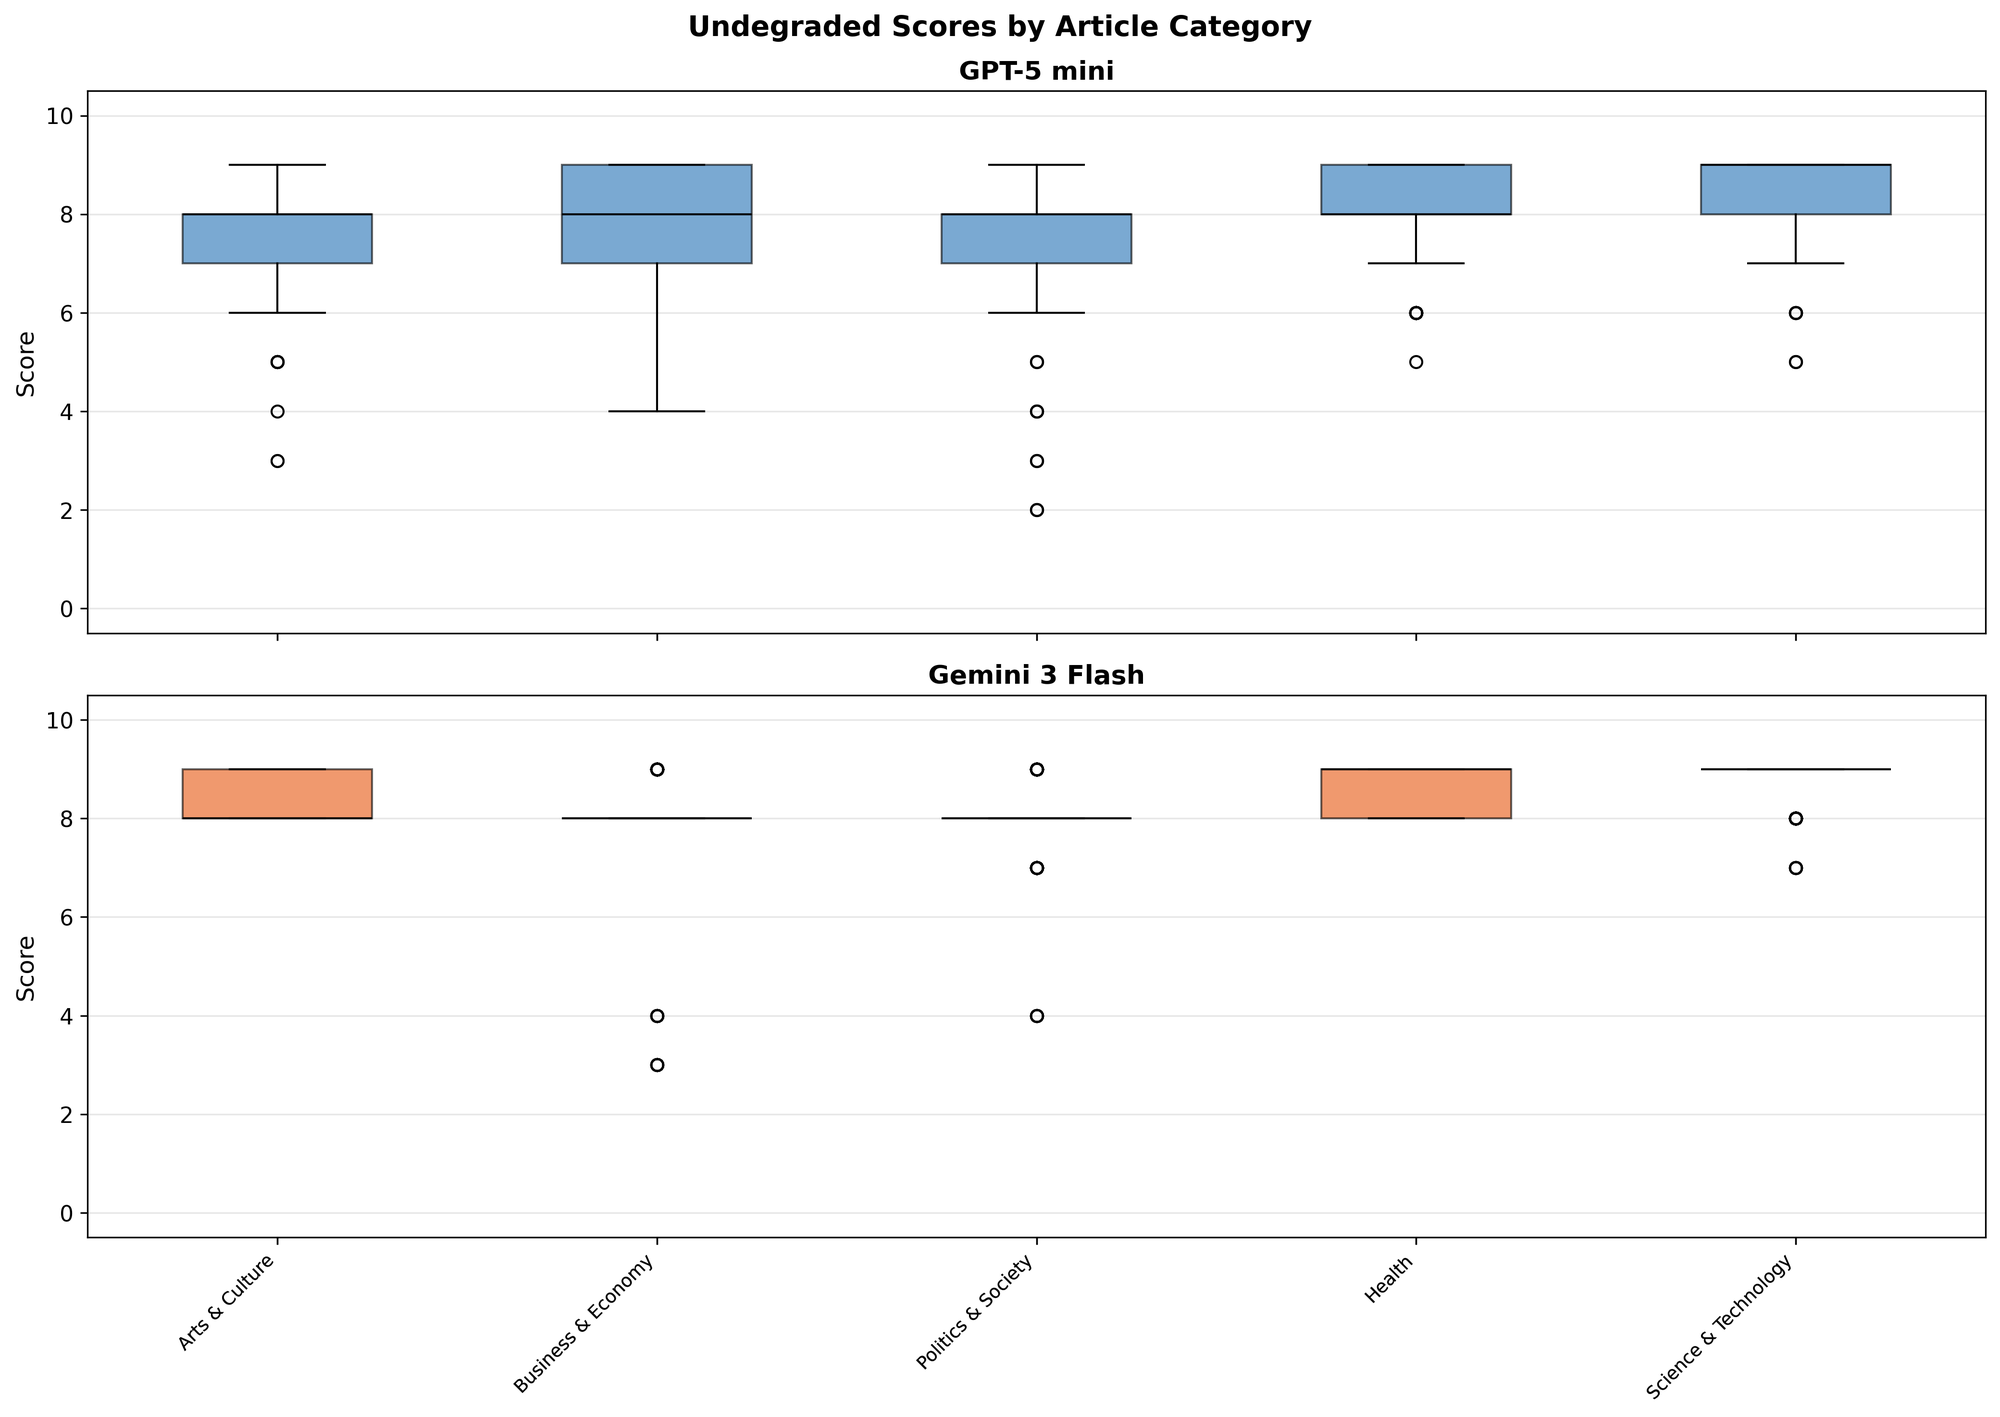
\includegraphics[width=\linewidth,keepaspectratio]{G13_category_effects.png}
\caption{Undegraded scores by article category. Both models score
Science \& Technology highest and Politics \& Society lowest despite
comparable editorial quality across categories.}
\label{fig:category}
\end{figure}

\subsection{Multiple Testing Correction}

Benjamini-Hochberg FDR correction across all 49 $p$-values leaves 47
significant at $\alpha = 0.05$. The two exceptions are the
article-length covariate for GPT-5~mini ($p_{\text{adj}} = 0.21$;
Section~\ref{sec:diagnostics}) and Mistral~7B's lexical slope
($p_{\text{adj}} = 0.49$; Appendix~Table~\ref{tab:slopes_app}).

% ══════════════════════════════════════════════════════════════
% 5. SCALING AND GENERALIZATION ACROSS MODELS
% ══════════════════════════════════════════════════════════════
\section{Scaling and Generalization Across Models}
\label{sec:multimodel}

Models range from 3.8B (Phi-4~mini) to 228B (MiniMax~M2P1)
parameters, all evaluated with the identical minimal prompt
(Table~\ref{tab:models}).

\subsection{Compression Across Models}

CRs range from 0.026 (Mistral~7B) to 0.685 (GPT-5~mini)
(Table~\ref{tab:compression}). Sub-10B models all achieve CR $< 0.30$;
models above 100B all achieve CR $\geq 0.42$
(Table~\ref{tab:compression}).

\subsection{Relationship Between Model Size and Compression}

Among nine open-weight models with known parameter counts, there is a
positive correlation between $\log_{10}(\text{parameters})$ and CR
(Pearson $r = 0.78$, $p = 0.013$; Table~\ref{tab:compression}).
However, the trend is noisy ($n = 9$) and non-monotonic:
MiniMax~M2P1 (228B) achieves a lower CR (0.42) than Qwen~2.5~14B
(0.45), and Gemma~2~9B achieves Spearman $\rho = 0.70$ despite a
modest CR of 0.30 (Table~\ref{tab:compression}), indicating model
size alone does not determine compression severity. Architecture,
training data, and RLHF procedures~\citep{rafailov2023direct} likely
contribute. We characterize this as a \emph{trend} rather than a
scaling law; confirmation across a broader model landscape is needed.

% ══════════════════════════════════════════════════════════════
% 6. MITIGATION STRATEGIES AND RESULTS
% ══════════════════════════════════════════════════════════════
\section{Mitigation Strategies \& Results}
\label{sec:mitigation}
\label{sec:mitresults}

We evaluate five strategies targeting different aspects of compression
(mathematical formulations in Appendix~\ref{app:mitigations}):
\begin{itemize}[nosep,leftmargin=*]
    \item \textbf{Quantile Normalization:} Maps the empirical
    distribution to a Uniform$[0, 10]$ or Beta$(2, 2)$ target via
    quantile matching~\citep{bolstad2003comparison}, preserving rank
    order.
    \item \textbf{Expected-Score Rescaling:} Replaces argmax with the
    probability-weighted expected score
    $\mathbb{E}[S]$~\citep{liu2023geval}.
    \item \textbf{Asymmetry Correction:} Adjusts $\mathbb{E}[S]$ by a
    skewness penalty~\citep{liu2023geval}. Cross-validation optimal
    $\alpha = 0.0$ reduces this entirely to expected-score rescaling.
    \item \textbf{Auxiliary Regression:} Trains supervised regressors
    on logprob-derived features to predict proxy ground truth.
    \item \textbf{Contrastive Anchor Prompting:} Prepends explicit scale
anchors (\eg ``0 = unreadable garbage'') to the system
prompt~\citep{zheng2023judging,liu2023geval}.
\end{itemize}

\begin{table}[htbp]
\centering
\caption{Mitigation comparison on nine logprob models. Range
Utilization (RU) = $(\max - \min)/10$; PA = Pairwise Accuracy.
Asymmetry Correction is omitted as it collapsed to Expected Score.}
\label{tab:mitcompare}
\begin{adjustbox}{max width=\columnwidth}
\begin{tabular}{@{}lcccc@{}}
\toprule
\textbf{Method} & \textbf{Spearman} $\rho$ & $\Delta\rho$ &
\textbf{RU} & \textbf{PA} \\
\midrule
Raw (baseline)                  & 0.458         & ---          & 0.689 & 0.518 \\
Quantile (Uniform)              & 0.458         & $+$0.000     & 0.922 & 0.518 \\
Expected score $\mathbb{E}[S]$  & 0.490         & $+$0.032     & 0.579 & 0.649 \\
Auxiliary Regressor             & \textbf{0.496}& \textbf{$+$0.038} & 0.919 & \textbf{0.702} \\
\bottomrule
\end{tabular}
\end{adjustbox}
\end{table}

\textbf{Results.} Post-hoc corrections provide modest benefits but do
not fundamentally fix the problem. Quantile normalization recovers the
full scale (RU: $0.689 \to 0.922$) while preserving rank order
exactly~\citep{bolstad2003comparison}. Expected-score rescaling
improves rank correlation ($\rho: 0.458 \to 0.490$) and pairwise
accuracy (PA: $0.518 \to 0.649$)~\citep{liu2023geval}, but further
shrinks the usable range (RU $\to 0.579$) because the underlying
logit distribution is already concentrated toward the centre of the
scale~\citep{rafailov2023direct}, so the probability-weighted
expectation moves away from integer endpoints.

Auxiliary regression yields the largest gains ($\rho \to 0.496$,
PA $\to 0.702$; Table~\ref{tab:mitcompare}) but requires supervised
training data. Contrastive anchor prompting yielded mixed results on
the two API models ($n = 200$ each): Gemini improved ($\Delta\rho =
+0.035$) while GPT-5~mini degraded ($\Delta\rho = -0.110$),
suggesting prompt engineering cannot reliably override deep-seated
distributional tendencies~\citep{rafailov2023direct}.

The maximum rank improvement ($\Delta\rho = +0.038$,
Table~\ref{tab:mitcompare}) demonstrates that rank-order information
is largely fixed at inference time.

% ══════════════════════════════════════════════════════════════
% 7. DISCUSSION
% ══════════════════════════════════════════════════════════════
\section{Discussion}
\label{sec:discussion}

\subsection{The Compression Effect}

Score compression is robust and reproducible across all eleven models.
GPT-5~mini and Gemini~3~Flash compress the effective range to
62--69\% of ideal without ever producing boundary scores; CRs across
all eleven models span 0.026--0.685 (Table~\ref{tab:compression},
Section~\ref{sec:results}). Calibrated simulations confirm this is
not a design artifact: an equivalent linear scorer would produce
hundreds of extreme scores (Section~\ref{sec:results};
Table~\ref{tab:dist}).

The compression is asymmetric and concave. Pristine texts receive mean
scores of 7.3--8.7 rather than 10 (Figure~\ref{fig:undegraded};
Table~\ref{tab:dist}); maximally degraded texts score well above the
expected floor. Significant quadratic terms in 34 of 44
axis$\times$model regressions confirm non-linearity
(Appendix~Table~\ref{tab:nonlin}, Figure~\ref{fig:residuals}).

The axis-specific sensitivity pattern reveals a systematic
psychometric blind spot: models respond aggressively to surface-level
manipulations (information deletion, grammatical errors) but are
comparatively insensitive to discourse coherence degradation
(Figure~\ref{fig:forest}; Appendix~Table~\ref{tab:slopes_app}).
Sentence shuffling destroys argumentative structure and entity-grid
transitions~\citep{barzilay2008modeling}, yet models barely adjust
their scores relative to sentence-level perturbations, suggesting that
LLM-based point-wise evaluation relies disproportionately on local,
token-level fluency signals rather than genuine document-level
reasoning~\citep{lapata2005automatic}.

\subsection{Absolute Scoring vs.\ Rank Ordering}

The stark dissociation between models' high rank-order correlations
(Spearman $\rho$ up to 0.80; Table~\ref{tab:compression}) and their
severe absolute compression ratios (CR as low as 0.026;
Sections~\ref{sec:results}--\ref{sec:multimodel}) has a clear
practical implication: models perceive the synthetic quality
gradients---they successfully order a degraded text below its intact
counterpart---but their translation of that preference into a single
absolute number is unreliable. When forced to produce a point estimate
without relative anchors, the model defaults toward the centre of its
learned output distribution, consistent with the mode-seeking property
of reverse KL-divergence in RLHF training~\citep{rafailov2023direct}.

This is also consistent with evidence that LLMs perform more
reliably as pairwise rankers than as absolute
scorers~\citep{zheng2023judging,liu2023geval}. It explains why
post-hoc rank corrections yield only modest gains ($\Delta\rho \leq
0.038$; Table~\ref{tab:mitcompare}): the rank information is largely
preserved; the problem is the loss of absolute calibration, which no
monotonic rescaling can fully recover
(Section~\ref{sec:calibration}).

\subsection{Linearity as Approximation}

The linear reference $S = 10(1 - \lambda)$ provides an interpretable
benchmark despite the empirically concave dose-response
(Figure~\ref{fig:doseresponse}). This choice is defensible on three
grounds. First, boundary-score absence is a model-free observation
requiring no reference function (Table~\ref{tab:dist}). Second,
affine, sigmoid, and isotonic calibrations all converge to nearly
identical curves (Section~\ref{sec:calibration},
Figure~\ref{fig:calibrecovery}), confirming residual non-linearity
beyond the affine is modest. Third, a concave true function would mean
our reported CRs \emph{understate} compression---our benchmark is
conservative by design.

\subsection{Axis-Specific Sensitivity}

Most models agree on axis sensitivity ordering: information deletion
is steepest; coherence or lexical disruption is shallowest
(Appendix~Table~\ref{tab:slopes_app}, Figure~\ref{fig:crossaxis}),
with exceptions (\eg Llama~3.1~8B peaks on grammar). The low
coherence sensitivity is particularly noteworthy: shuffling sentences
destroys argumentative flow and entity
transitions~\citep{barzilay2008modeling} while preserving all surface
features, suggesting models weight local, sentence-level quality over
global discourse structure~\citep{lapata2005automatic}.

\subsection{Systematic Inter-Model Bias}

Despite high agreement ($r = 0.836$; Figure~\ref{fig:scatter}),
Gemini~3~Flash scores one point higher than GPT-5~mini: a
\emph{systematic} offset (rank-biserial $r = 0.705$; Gemini scores
higher on 85\% of disagreements; Section~\ref{sec:intermodel},
Figure~\ref{fig:paireddiff}). Scores from different providers are not
interchangeable---a threshold calibrated on GPT scores would
systematically fail on Gemini scores
(Section~\ref{sec:intermodel}; Table~\ref{tab:compression}). This is
analogous to inter-rater scale-use differences documented in human
rating studies~\citep{guilford1954psychometric}.

\subsection{Reliability}

Both API models achieve ICC $> 0.90$; ten of eleven models achieve
ICC $> 0.70$ (Appendix~Table~\ref{tab:icc_app}). Compression is a
stable, deterministic property of the scoring function, not a noise
artifact (Appendix~Table~\ref{tab:icc_app}). This also confirms that
the fixed sampling behaviour of GPT-5~mini does not introduce
materially higher variance relative to temperature-0.0 models
(Appendix~Table~\ref{tab:icc_app}).

\subsection{Relationship to Prior Work on Calibration}

Surveys of supervised AES demonstrate that models fine-tuned on
domain-specific training data can closely match target human scoring
distributions~\citep{ke2019automated}. Similarly, evaluation
frameworks providing detailed rubrics or binary-like scales report
smaller gaps between absolute scoring and relative
ranking~\citep{liu2023geval}. These findings are not in conflict with
ours: they apply to specialist models or constrained scales, and each
requires substantial additional supervision or prompt
engineering~\citep{ke2019automated,liu2023geval}. Our study measures
the intrinsic zero-shot calibration of general-purpose instruct
models---the setting describing the overwhelming majority of
LLM-as-judge deployments in practice~\citep{zheng2023judging}. The
evidence that compression \emph{can} be reduced under ideal
conditions~\citep{ke2019automated} makes its persistence in
uncalibrated deployment all the more practically significant.

\subsection{Implications}
\begin{enumerate}[nosep]
    \item \textbf{Score calibration is necessary.} Raw LLM scores
    should not be treated as ground
    truth~\citep{liu2023geval,zheng2023judging}. Quantile
    normalization is a simple, model-agnostic range-recovery
    approach~\citep{bolstad2003comparison}
    (Section~\ref{sec:mitigation}).
    \item \textbf{Model-specific thresholds.} A score of 7 from
    GPT-5~mini is not equivalent to a 7 from Gemini~3~Flash
    (Section~\ref{sec:intermodel}; Figure~\ref{fig:paireddiff}).
    \item \textbf{Ordinal, not interval.} Score spacing is
    non-uniform~\citep{stevens1971issues}; effective endpoints differ
    from nominal ones (Table~\ref{tab:dist}).
    \item \textbf{Axis awareness.} LLMs are substantially less
    sensitive to coherence-level quality variation
    (Figure~\ref{fig:forest};
    Appendix~Table~\ref{tab:slopes_app}).
    \item \textbf{Post-hoc corrections help modestly.} Maximum
    $\Delta\rho = +0.038$ (Table~\ref{tab:mitcompare}) confirms
    quality rankings are largely fixed at inference
    time~\citep{rafailov2023direct}.
    \item \textbf{Prompt-level interventions are unreliable.}
    Contrastive anchoring produced inconsistent results
    (Section~\ref{sec:mitigation}) and is not a robust
    mitigation~\citep{rafailov2023direct}.
    \item \textbf{Model scale matters, noisily.} Larger models tend
    toward less compression (Section~\ref{sec:multimodel}), but
    exceptions exist (Table~\ref{tab:compression}); size alone does
    not guarantee well-calibrated scores.
\end{enumerate}

% ══════════════════════════════════════════════════════════════
% 8. CONCLUSION
% ══════════════════════════════════════════════════════════════
\section{Conclusion}
\label{sec:conclusion}

Score compression is a robust, reproducible phenomenon across eleven
models (3.8B--228B parameters, multiple providers), confirmed through
$\sim$99{,}000 evaluations
(Sections~\ref{sec:results}--\ref{sec:multimodel}). CRs range from
0.026 to 0.685 and correlate positively with model size ($r = 0.78$;
Table~\ref{tab:compression}, Section~\ref{sec:multimodel}), with
notable exceptions. GPT-5~mini and Gemini~3~Flash both compress the
effective range to 62--69\% of ideal (Section~\ref{sec:results};
Table~\ref{tab:compression}).

Among five mitigation strategies (Section~\ref{sec:mitigation}),
quantile normalization~\citep{bolstad2003comparison} efficiently
recovers distributional range, expected-score
rescaling~\citep{liu2023geval} modestly improves rank correlation,
auxiliary regression gives the best pairwise accuracy gains, and
contrastive anchor prompting~\citep{zheng2023judging,liu2023geval}
produces inconsistent results; the maximum $\Delta\rho = +0.038$
(Table~\ref{tab:mitcompare}) confirms quality rankings are largely
baked in at inference time~\citep{rafailov2023direct}.

Our work is the first to quantify distributional bias against an
algebraically defined ground truth across eleven models, four
psychometric axes~\citep{attali2006automated,mcnamara2010linguistic},
and five mitigation strategies. The title reflects the core finding:
no one gets an A---LLMs resist assigning top marks just as they resist
failing grades (Table~\ref{tab:dist}), funneling evaluations into a
safe middle range driven by the mode-seeking properties of alignment
training~\citep{rafailov2023direct}. Understanding and correcting this
distributional bias is essential for any application relying on
LLM-generated quality ratings~\citep{zheng2023judging,liu2023geval}.

% ══════════════════════════════════════════════════════════════
% LIMITATIONS
% ══════════════════════════════════════════════════════════════
\section*{Limitations}

First, degradation axes, though designed to be orthogonal
(Section~\ref{sec:axis_justification}), may have residual
correlations (\eg information deletion may incidentally affect
coherence~\citep{barzilay2008modeling}). Second, the corpus is
English expository text from a single source; generalization to other
languages, genres, or domains requires further
investigation~\citep{mcnamara2010linguistic}. Third, the broader
model landscape---particularly commercial models without logprob
access---may show further variation
(Section~\ref{sec:mitigation}; Table~\ref{tab:models}).

Fourth, the temperature asymmetry (GPT-5~mini with an unsupported
temperature parameter, Gemini~3~Flash at temperature 0.0) is a
meaningful confound. However, a temperature-driven explanation
predicts GPT should compress \emph{more} than Gemini---the opposite
of what we observe (CR: 0.685 vs.\ 0.620;
Table~\ref{tab:compression}). GPT's ICC remains excellent at 0.926
(Appendix~Table~\ref{tab:icc_app}), and majority-vote aggregation
yields near-identical mean scores (mean absolute deviation $< 0.05$).
Nevertheless, future work should compare models at matched
temperatures where API constraints permit.

Fifth, logprob-based mitigations are evaluated on only the nine models
that expose token probabilities; contrastive prompting on only two API
models. Controlled comparisons on matching model sets
(Table~\ref{tab:mitcompare}) address this.

Sixth, the reference $S = 10(1 - \lambda)$ assumes linear quality
degradation. This is a mathematical convenience, not a perceptual
claim. Crucially, the boundary-score absence finding
(Section~\ref{sec:results}; Table~\ref{tab:dist}) is entirely
independent of this assumption; under a concave ground truth, our CRs
would be understated, making our benchmark conservative.

Seventh, the intentionally minimal scoring prompt measures intrinsic
calibration bias but leaves untested more elaborate
designs---chain-of-thought, decomposed evaluation, fine-grained
rubrics~\citep{liu2023geval}---which may yield different results. Our
contrastive anchor experiment (Section~\ref{sec:mitresults}) suggests
the bias is not purely prompt-driven~\citep{rafailov2023direct}, but
further investigation is warranted.

Eighth, our study evaluates general-purpose instruct models in a
zero-shot setting~\citep{zheng2023judging}. Prior work suggests that
fine-tuning models specifically for evaluation tasks can achieve high
distributional alignment with target human
ratings~\citep{ke2019automated}. Whether such training eliminates or
merely attenuates the bias, and at what cost to generality, remains an
important open question.

% ══════════════════════════════════════════════════════════════
% ETHICAL CONSIDERATIONS
% ══════════════════════════════════════════════════════════════
\section*{Ethical Considerations}

Score compression has direct ethical implications for LLM deployment
in high-stakes evaluation---essay grading, recruitment screening,
content moderation~\citep{zheng2023judging}. Naive threshold-based
decisions are inherently miscalibrated
(Section~\ref{sec:results}; Section~\ref{sec:calibration}): an
institution requiring a score of 9 to award a scholarship, or 8 to
pass a resume screen, will arbitrarily reject qualified candidates due
to ceiling compression (Table~\ref{tab:dist}), while floor
compression may shield poor submissions from necessary remediation.

Inter-model bias compounds this (Section~\ref{sec:intermodel}):
Gemini~3~Flash scores roughly one point higher than GPT-5~mini on
identical texts (Figure~\ref{fig:paireddiff};
Table~\ref{tab:compression}). Institutions switching or mixing LLM
evaluators will create systematic, opaque inequities across evaluated
individuals~\citep{guilford1954psychometric}.

Post-hoc mitigations (Section~\ref{sec:mitigation}) recover only
partial calibration and cannot retrieve discriminative signals the
underlying model failed to capture
(Section~\ref{sec:calibration}). LLM-generated scores are at best
ordinal signals~\citep{stevens1971issues}; deploying them in
automated decision-making requires rigorous, context-specific
validation against domain-expert baselines~\citep{ke2019automated}.

% ══════════════════════════════════════════════════════════════
% REFERENCES
% ══════════════════════════════════════════════════════════════
\begin{thebibliography}{25}
\bibitem[Attali and Burstein(2006)]{attali2006automated}
Yigal Attali and Jill Burstein.
\newblock 2006.
\newblock Automated essay scoring with {e-rater}{\textregistered} {V.2}.
\newblock \emph{Journal of Technology, Learning, and Assessment}, 4(3):1--21.

\bibitem[Barzilay and Lapata(2008)]{barzilay2008modeling}
Regina Barzilay and Mirella Lapata.
\newblock 2008.
\newblock Modeling local coherence: An entity-based approach.
\newblock \emph{Computational Linguistics}, 34(1):1--34.

\bibitem[Bolstad et~al.(2003)]{bolstad2003comparison}
Benjamin~M. Bolstad, Rafael~A. Irizarry, Magnus {\AA}strand, and
Terence~P. Speed.
\newblock 2003.
\newblock A comparison of normalization methods for high density
oligonucleotide array data based on variance and bias.
\newblock \emph{Bioinformatics}, 19(2):185--193.
\newblock \url{https://doi.org/10.1093/bioinformatics/19.2.185}.

\bibitem[Guilford(1954)]{guilford1954psychometric}
Joy~Paul Guilford.
\newblock 1954.
\newblock \emph{Psychometric Methods}.
\newblock McGraw-Hill, New York, 2nd edition.

\bibitem[Ke and Ng(2019)]{ke2019automated}
Zihao Ke and Vincent Ng.
\newblock 2019.
\newblock Automated essay scoring: A survey of the state of the art.
\newblock In \emph{Proceedings of the 28th International Joint Conference
on Artificial Intelligence}, pages 6300--6308.
\newblock \url{https://doi.org/10.24963/ijcai.2019/879}.

\bibitem[Kocmi and Federmann(2023)]{kocmi2023large}
Tom Kocmi and Christian Federmann.
\newblock 2023.
\newblock Large language models are state-of-the-art evaluators of
translation quality.
\newblock In \emph{Proceedings of the 24th Annual Conference of the
European Association for Machine Translation}, pages 193--203.
\newblock \url{https://aclanthology.org/2023.eamt-1.19}.

\bibitem[Lapata and Barzilay(2005)]{lapata2005automatic}
Mirella Lapata and Regina Barzilay.
\newblock 2005.
\newblock Automatic evaluation of text coherence: Models and representations.
\newblock In \emph{Proceedings of the 19th International Joint Conference
on Artificial Intelligence}, pages 1085--1090.

\bibitem[Glava{\v{s}} and {\v{S}}tajner(2015)]{glavas2015simplifying}
Goran Glava{\v{s}} and Sanja {\v{S}}tajner.
\newblock 2015.
\newblock Simplifying lexical simplification: Do we need simplified corpora?
\newblock In \emph{Proceedings of the 53rd Annual Meeting of the Association
for Computational Linguistics and the 7th International Joint Conference on
Natural Language Processing (Volume 2: Short Papers)}, pages 63--68.

\bibitem[Li et~al.(2025)]{li2025preference}
Dawei Li, Renliang Sun, et~al.
\newblock 2025.
\newblock Preference leakage: A contamination problem in {LLM}-as-a-judge.
\newblock \emph{arXiv preprint arXiv:2502.01534}.
\newblock \url{https://arxiv.org/abs/2502.01534}.

\bibitem[Liu et~al.(2023)]{liu2023geval}
Yang Liu, Dan Iter, Yichong Xu, Shuohang Wang, Ruochen Xu, and Chenguang
Zhu.
\newblock 2023.
\newblock G-{E}val: {NLG} evaluation using {GPT-4} with better human
alignment.
\newblock In \emph{Proceedings of the 2023 Conference on Empirical Methods
in Natural Language Processing}, pages 2511--2522.
\newblock \url{https://doi.org/10.18653/v1/2023.emnlp-main.153}.

\bibitem[McNamara et~al.(2010)]{mcnamara2010linguistic}
Danielle~S. McNamara, Scott~A. Crossley, and Philip~M. McCarthy.
\newblock 2010.
\newblock Linguistic features of writing quality.
\newblock \emph{Written Communication}, 27(1):57--86.

\bibitem[Qiang et~al.(2020)]{qiang2020lexical}
Jipeng Qiang, Yun Li, Yi Zhu, Yunhao Yuan, and Xindong Wu.
\newblock 2020.
\newblock Lexical simplification with pretrained encoders.
\newblock In \emph{Proceedings of the AAAI Conference on Artificial
Intelligence}, 34(05):8649--8656.

\bibitem[Rafailov et~al.(2023)]{rafailov2023direct}
Rafael Rafailov, Archit Sharma, Eric Mitchell, Christopher~D. Manning,
Stefano Ermon, and Chelsea Finn.
\newblock 2023.
\newblock Direct preference optimization: Your language model is secretly
a reward model.
\newblock \emph{Advances in Neural Information Processing Systems}, 36.

\bibitem[Ribeiro et~al.(2020)]{ribeiro2020beyond}
Marco~Tulio Ribeiro, Tongshuang Wu, Carlos Guestrin, and Sameer Singh.
\newblock 2020.
\newblock Beyond accuracy: Behavioral testing of {NLP} models with
{CheckList}.
\newblock In \emph{Proceedings of the 58th Annual Meeting of the
Association for Computational Linguistics}, pages 4902--4912.

\bibitem[Shi et~al.(2024)]{shi2024judging}
Congcong Shi et~al.
\newblock 2024.
\newblock Judging the judges: A systematic study of position bias in
{LLM}-as-a-judge.
\newblock In \emph{Proceedings of IJCNLP 2025}.
\newblock \url{https://arxiv.org/abs/2406.07791}.

\bibitem[Stevens(1971)]{stevens1971issues}
Stanley~S. Stevens.
\newblock 1971.
\newblock Issues in psychophysical measurement.
\newblock \emph{Psychological Review}, 78(5):426--450.
\newblock \url{https://doi.org/10.1037/h0031324}.

\bibitem[Wang et~al.(2024)]{wang2024large}
Peiyi Wang, Lei Li, Liang Chen, Zefan Cai, Dawei Zhu, Binghuai Lin,
Yunbo Cao, Lingpeng Kong, Qi Liu, Tianyu Liu, and Zhifang Sui.
\newblock 2024.
\newblock Large language models are not fair evaluators.
\newblock In \emph{Proceedings of the 62nd Annual Meeting of the
Association for Computational Linguistics}, pages 9440--9450.
\newblock \url{https://aclanthology.org/2024.acl-long.511/}.

\bibitem[Zheng et~al.(2023)]{zheng2023judging}
Lianmin Zheng, Wei-Lin Chiang, Ying Sheng, Siyuan Zhuang, Zhanghao Wu,
Yonghao Zhuang, Zi Lin, Zhuohan Li, Dacheng Li, Eric~P. Xing, Hao
Zhang, Joseph~E. Gonzalez, and Ion Stoica.
\newblock 2023.
\newblock Judging {LLM}-as-a-judge with {MT-Bench} and {Chatbot Arena}.
\newblock \emph{Advances in Neural Information Processing Systems}, 36.
\newblock \url{https://proceedings.neurips.cc/paper_files/paper/2023/hash/91f18a1287b398d378ef22505bf41832-Abstract-Datasets_and_Benchmarks.html}.
\end{thebibliography}

% ══════════════════════════════════════════════════════════════
% APPENDIX
% ══════════════════════════════════════════════════════════════
\appendix
\section{Mitigation Formulas}
\label{app:mitigations}

\textbf{Expected-Score Rescaling.} For models returning token-level
log-probabilities, the argmax score is replaced by the
probability-weighted expected value~\citep{liu2023geval}:
\begin{equation}
    \hat{S} = \mathbb{E}[S] = \sum_{k=0}^{10} k \cdot p(k)
\end{equation}
where $p(k)$ is the softmax probability of score token $k$.

\textbf{Asymmetry Correction.} An extension of expected-score
rescaling~\citep{liu2023geval} correcting for distribution
skewness~\citep{stevens1971issues}:
\begin{equation}
    \hat{S}_{\text{adj}} = \mathbb{E}[S] - \alpha \cdot
    \text{skewness}(p)
\end{equation}
with $\alpha$ tuned via five-fold cross-validation. In our
experiments, the optimal $\alpha$ was 0.0 for all models, reducing
this method entirely to expected-score rescaling~\citep{liu2023geval}.

\section{Mixed-Effects Model: Key Coefficients}
\label{app:mixed}

Table~\ref{tab:mixedeffects_app} reports all fixed-effect coefficients
from the three-way model described in Section~\ref{sec:mixedeffects}.
Reference levels are the Grammar axis and GPT-5~mini. All three-way
Level $\times$ Axis $\times$ Model interactions were significant
($p < 0.001$); the largest is reported in the main text
(Section~\ref{sec:mixedeffects}).
Random-effects estimates are listed at the bottom of the table.

\begin{table}[H]
\centering
\caption{Fixed-effect coefficients for the three-way linear
mixed-effects model. ``---'' indicates the value is subsumed in the
reference level intercept. All terms marked $p < 0.001$ were
significant after Benjamini-Hochberg correction.}
\label{tab:mixedeffects_app}
\small
\begin{adjustbox}{max width=\columnwidth}
\begin{tabular}{@{}lrrl@{}}
\toprule
\textbf{Term} & $\hat{\beta}$ & $z$ & $p$ \\
\midrule
\multicolumn{4}{l}{\textit{Fixed effects}} \\
Degradation level ($\lambda$) & $-4.76$ & $-45.6$ & $<10^{-300}$ \\
Model: Gemini vs.\ GPT (intercept) & $+0.07$ & --- & $0.25$ (n.s.) \\
Axis: Grammar (intercept reduction) & $-1.49$ & $-25.1$ & $<0.001$ \\
Axis: Coherence & --- & --- & significant \\
Axis: Information & --- & --- & significant \\
Axis: Lexical & --- & --- & significant \\
Level $\times$ Lexical $\times$ Gemini & $+1.93$ & $+11.2$ & $<0.001$ \\
All other Level $\times$ Axis $\times$ Model & --- & --- & all $<0.001$ \\
\midrule
\multicolumn{4}{l}{\textit{Random effects (article level)}} \\
Intercept variance & \multicolumn{3}{l}{$0.54$} \\
Slope variance & \multicolumn{3}{l}{$0.49$} \\
\bottomrule
\end{tabular}
\end{adjustbox}
\end{table}

\section{Extended Results Tables}
\label{app:diagnostics}

\begin{table}[H]
\centering
\caption{Regression slopes ($\beta_1$) of score on degradation level.
All $p < 0.001$ except Mistral~7B lexical ($p = 0.49$, shown in
gray).}
\label{tab:slopes_app}
\small
\begin{adjustbox}{max width=\columnwidth}
\begin{tabular}{@{}lccccc@{}}
\toprule
\textbf{Model} & \textbf{Grammar} & \textbf{Coherence} &
\textbf{Information} & \textbf{Lexical} & \textbf{Mean} \\
\midrule
GPT-5 mini     & $-6.82$ & $-4.78$ & $-7.87$ & $-6.38$ & $-6.46$ \\
Gemini 3 Flash & $-6.81$ & $-5.58$ & $-7.05$ & $-5.26$ & $-6.18$ \\
GPT-OSS 120B   & $-5.16$ & $-3.36$ & $-6.08$ & $-4.55$ & $-4.79$ \\
Qwen 2.5 14B   & $-5.97$ & $-1.21$ & $-6.64$ & $-4.46$ & $-4.57$ \\
MiniMax M2P1   & $-5.59$ & $-2.04$ & $-5.56$ & $-3.73$ & $-4.23$ \\
Gemma 2 9B     & $-4.77$ & $-2.02$ & $-3.63$ & $-1.69$ & $-3.03$ \\
Phi-4 14B      & $-2.77$ & $-0.47$ & $-3.09$ & $-0.90$ & $-1.81$ \\
Llama 3.1 8B   & $-3.70$ & $-0.69$ & $-1.25$ & $-0.65$ & $-1.57$ \\
Phi-4 mini     & $-1.12$ & $-0.47$ & $-1.35$ & $-0.23$ & $-0.79$ \\
Qwen 2.5 7B    & $-0.75$ & $-0.54$ & $-0.84$ & $-0.22$ & $-0.59$ \\
Mistral 7B     & $-0.41$ & $-0.28$ & $-0.41$ & \color{gray}{$-0.03$} & $-0.28$ \\
\bottomrule
\end{tabular}
\end{adjustbox}
\end{table}

\begin{table}[H]
\centering
\caption{Calibration recovery on held-out test set. RMSE computed
against $S^* = 10(1 - \lambda)$.}
\label{tab:calibration_app}
\begin{adjustbox}{max width=\columnwidth}
\begin{tabular}{@{}llcccc@{}}
\toprule
\textbf{Model} & \textbf{Calib.} & \textbf{RMSE} &
$\Delta$\textbf{RMSE} & \textbf{Kendall} $\tau$ &
\textbf{Spearman} $\rho$ \\
\midrule
\multirow{4}{*}{GPT-5 mini}
    & Raw      & 2.51 & ---    & 0.629 & 0.741 \\
    & Affine   & 1.88 & $-$25\% & 0.629 & 0.741 \\
    & Sigmoid  & 1.86 & $-$26\% & 0.629 & 0.741 \\
    & Isotonic & 1.85 & $-$26\% & 0.629 & 0.741 \\
\midrule
\multirow{4}{*}{Gemini 3 Flash}
    & Raw      & 1.94 & ---    & 0.684 & 0.782 \\
    & Affine   & 1.74 & $-$10\% & 0.684 & 0.782 \\
    & Sigmoid  & 1.74 & $-$10\% & 0.684 & 0.782 \\
    & Isotonic & 1.73 & $-$11\% & 0.684 & 0.782 \\
\bottomrule
\end{tabular}
\end{adjustbox}
\end{table}

\begin{table}[H]
\centering
\caption{Intra-condition reliability ICC(1,1) by axis.}
\label{tab:icc_app}
\small
\begin{adjustbox}{max width=\columnwidth}
\begin{tabular}{@{}lccccc@{}}
\toprule
\textbf{Model} & \textbf{Grammar} & \textbf{Coherence} &
\textbf{Info} & \textbf{Lexical} & \textbf{Overall} \\
\midrule
GPT-5 mini     & 0.963 & 0.850 & 0.925 & 0.897 & \textbf{0.926} \\
Gemini 3 Flash & 0.950 & 0.844 & 0.913 & 0.890 & \textbf{0.905} \\
GPT-OSS 120B   & 0.914 & 0.566 & 0.777 & 0.718 & 0.751 \\
Qwen 2.5 14B   & 0.845 & 0.605 & 0.856 & 0.744 & 0.849 \\
MiniMax M2P1   & 0.394 & 0.181 & 0.422 & 0.359 & 0.433 \\
Gemma 2 9B     & 0.891 & 0.823 & 0.852 & 0.873 & 0.888 \\
Phi-4 14B      & 0.765 & 0.702 & 0.811 & 0.794 & 0.826 \\
Llama 3.1 8B   & 0.716 & 0.689 & 0.711 & 0.767 & 0.805 \\
Phi-4 mini     & 0.619 & 0.734 & 0.759 & 0.778 & 0.719 \\
Qwen 2.5 7B    & 0.722 & 0.612 & 0.740 & 0.807 & 0.722 \\
Mistral 7B     & 0.717 & 0.663 & 0.726 & 0.880 & 0.745 \\
\bottomrule
\end{tabular}
\end{adjustbox}
\end{table}

\begin{table}[H]
\centering
\caption{$F$-statistic for quadratic term. Bold = significant ($F >
3.84$, $p < 0.05$); ``---'' = $F < 1$.}
\label{tab:nonlin}
\small
\begin{adjustbox}{max width=\columnwidth}
\begin{tabular}{@{}lcccc@{}}
\toprule
\textbf{Model} & \textbf{Grammar} & \textbf{Coherence} &
\textbf{Info} & \textbf{Lexical} \\
\midrule
GPT-5 mini     & \textbf{3{,}556} & \textbf{110} & \textbf{1{,}640} & \textbf{1{,}335} \\
Gemini 3 Flash & \textbf{1{,}757} & \textbf{463} & \textbf{192}     & \textbf{382}     \\
GPT-OSS 120B   & \textbf{880}     & \textbf{49}  & \textbf{120}     & \textbf{317}     \\
Qwen 2.5 14B   & \textbf{1{,}683} & ---          & \textbf{86}      & ---              \\
MiniMax M2P1   & \textbf{254}     & \textbf{17}  & \textbf{21}      & \textbf{29}      \\
Gemma 2 9B     & \textbf{73}      & \textbf{25}  & \textbf{63}      & \textbf{33}      \\
Phi-4 14B      & \textbf{63}      & ---          & \textbf{279}     & ---              \\
Llama 3.1 8B   & \textbf{96}      & \textbf{13}  & 7                & 10               \\
Phi-4 mini     & 3                & ---          & \textbf{105}     & 8                \\
Qwen 2.5 7B    & 2                & ---          & \textbf{44}      & ---              \\
Mistral 7B     & \textbf{14}      & ---          & \textbf{45}      & \textbf{19}      \\
\bottomrule
\end{tabular}
\end{adjustbox}
\end{table}

\begin{table}[H]
\centering
\caption{Kendall's $\tau$ between degradation level and score. All $p
< 10^{-4}$ except Mistral~7B lexical ($\tau = -0.005$, $p = 0.49$).}
\label{tab:tau}
\small
\begin{adjustbox}{max width=\columnwidth}
\begin{tabular}{@{}lcccc@{}}
\toprule
\textbf{Model} & \textbf{Grammar} & \textbf{Coherence} &
\textbf{Info} & \textbf{Lexical} \\
\midrule
GPT-5 mini     & $-0.733$ & $-0.568$ & $-0.827$ & $-0.675$ \\
Gemini 3 Flash & $-0.818$ & $-0.636$ & $-0.818$ & $-0.661$ \\
GPT-OSS 120B   & $-0.673$ & $-0.408$ & $-0.700$ & $-0.528$ \\
Qwen 2.5 14B   & $-0.708$ & $-0.382$ & $-0.761$ & $-0.559$ \\
MiniMax M2P1   & $-0.487$ & $-0.270$ & $-0.516$ & $-0.420$ \\
Gemma 2 9B     & $-0.768$ & $-0.585$ & $-0.747$ & $-0.524$ \\
Phi-4 14B      & $-0.700$ & $-0.264$ & $-0.716$ & $-0.375$ \\
Llama 3.1 8B   & $-0.605$ & $-0.358$ & $-0.506$ & $-0.315$ \\
Phi-4 mini     & $-0.265$ & $-0.136$ & $-0.348$ & $-0.058$ \\
Qwen 2.5 7B    & $-0.351$ & $-0.267$ & $-0.399$ & $-0.128$ \\
Mistral 7B     & $-0.172$ & $-0.129$ & $-0.181$ & $-0.005$ \\
\bottomrule
\end{tabular}
\end{adjustbox}
\end{table}

\section{Additional Figures}
\label{app:figures}

\begin{figure}[htbp]
\centering
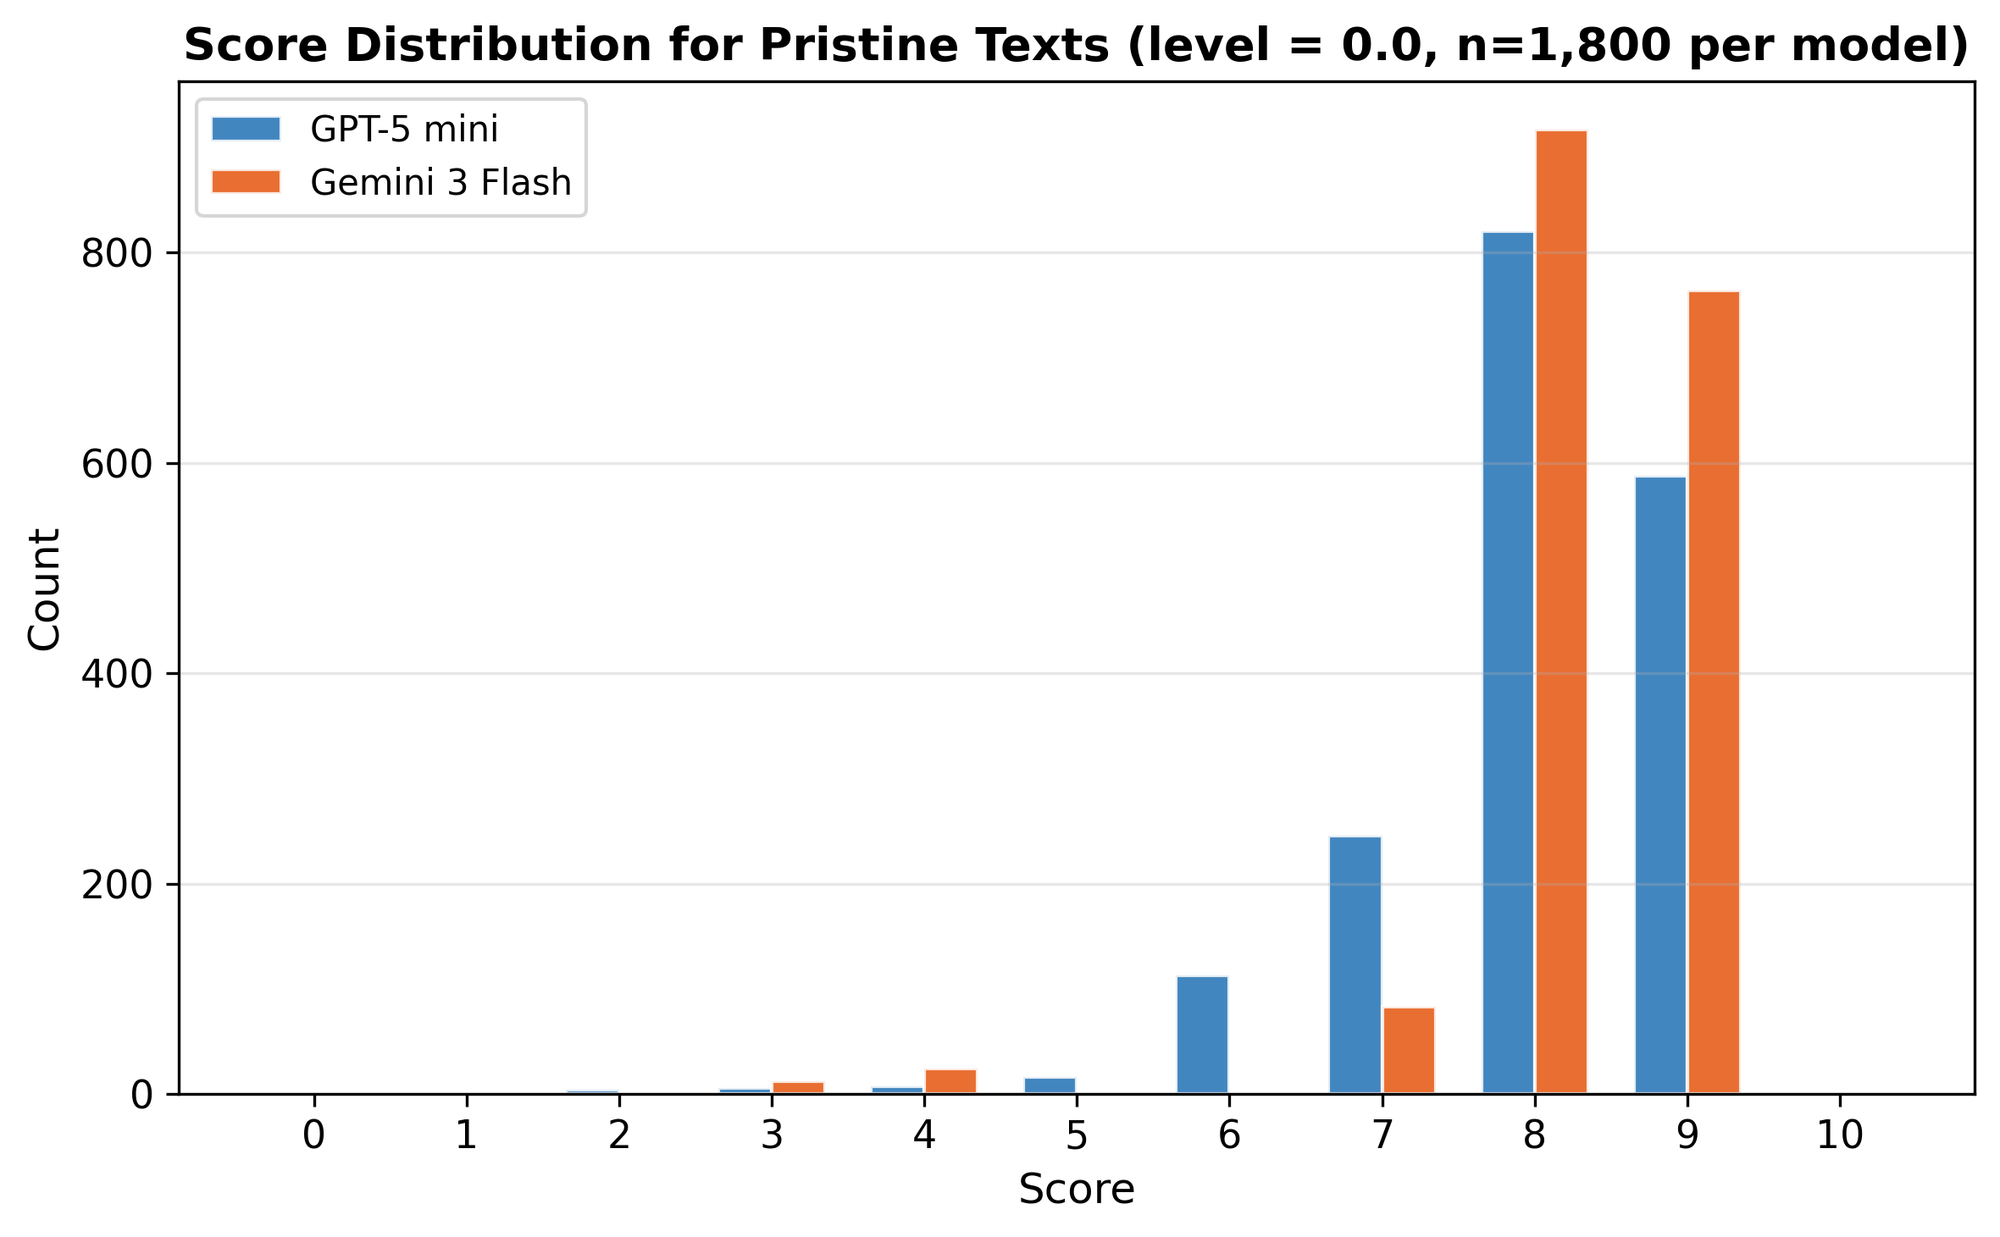
\includegraphics[width=\linewidth]{G4_undegraded_dist.png}
\caption{Score distributions for pristine ($\lambda = 0.0$) texts
only ($n = 1{,}800$ per model). All models concentrate scores in a
narrow top-of-scale band; most never assign 10 to expert-authored
articles.}
\label{fig:undegraded}
\end{figure}

\begin{figure}[htbp]
\centering
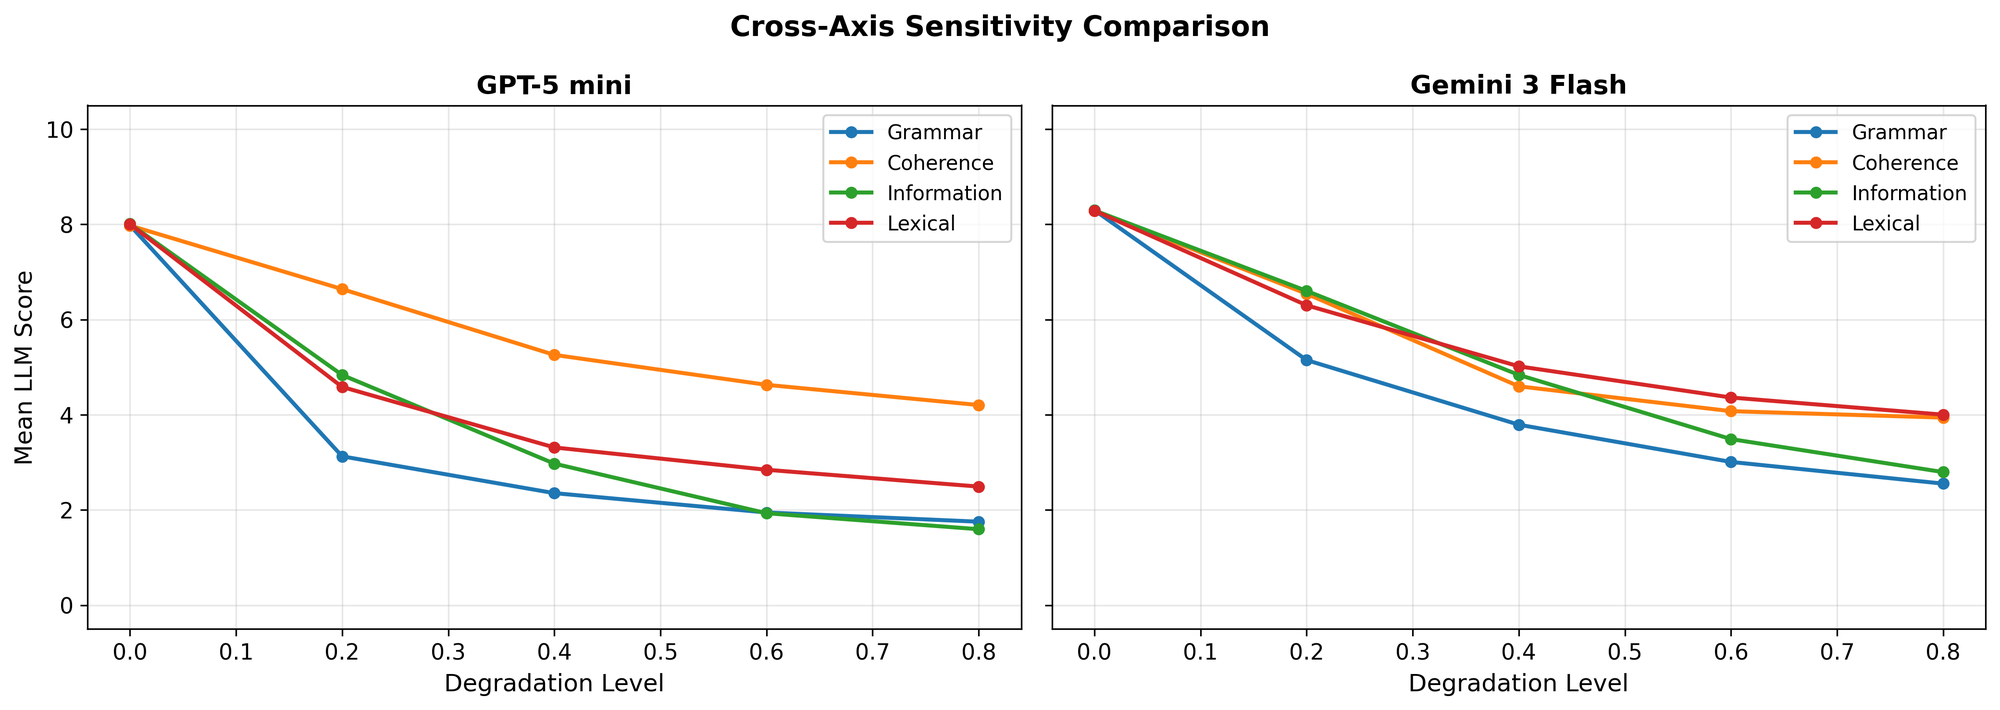
\includegraphics[width=\linewidth]{G2_cross_axis.png}
\caption{Cross-axis sensitivity per model. Both models are most
sensitive to information deletion; GPT-5~mini least to coherence,
Gemini~3~Flash least to lexical degradation.}
\label{fig:crossaxis}
\end{figure}

\begin{figure}[htbp]
\centering
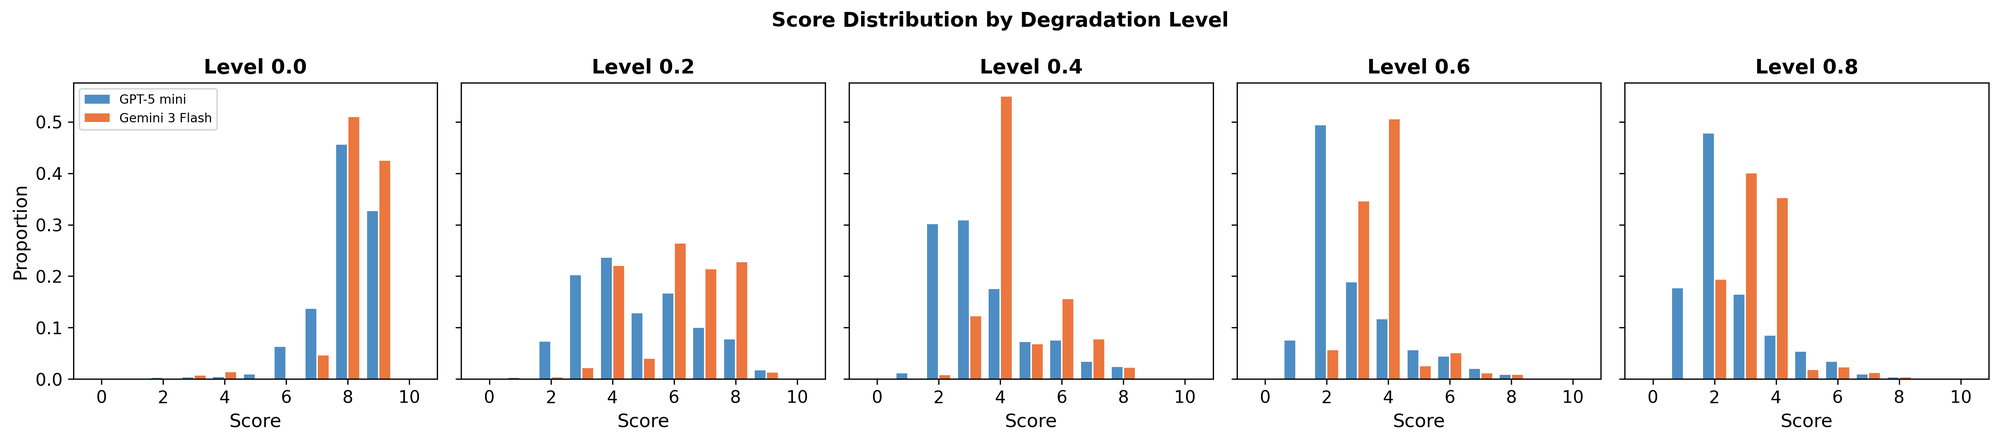
\includegraphics[width=\linewidth]{G5_per_level_dist.png}
\caption{Score distributions by degradation level. At $\lambda =
0.0$, scores concentrate at 8--9; by $\lambda = 0.8$, at 2--4.}
\label{fig:perlevel}
\end{figure}

\begin{figure}[htbp]
\centering
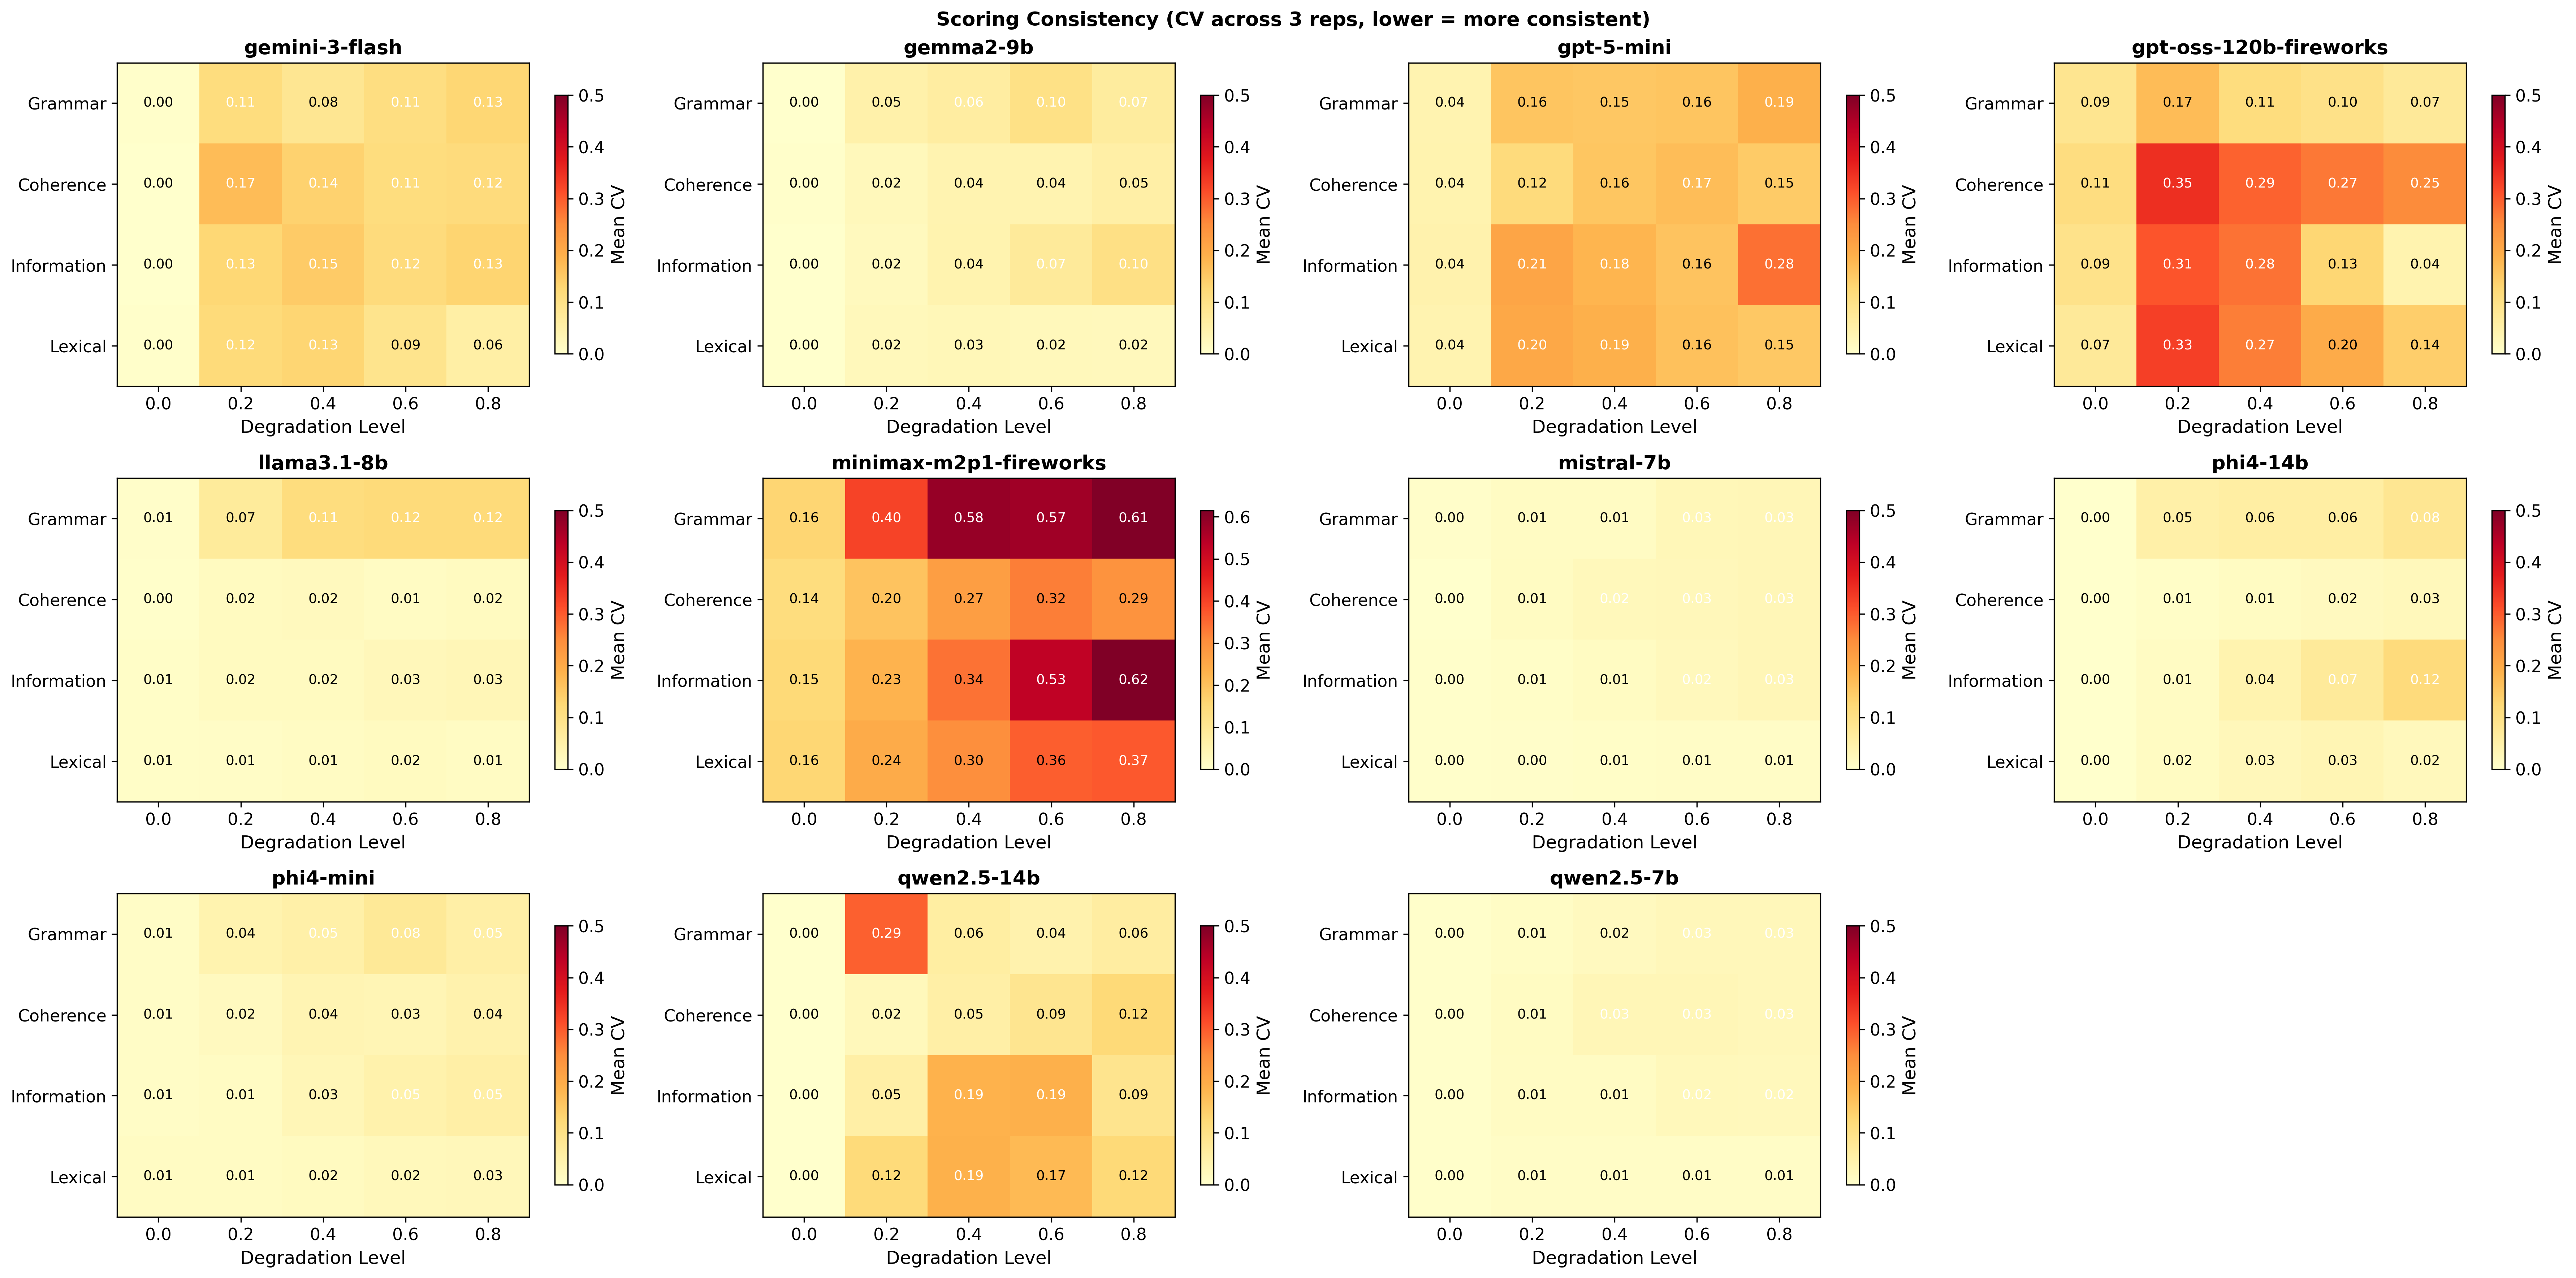
\includegraphics[width=\linewidth,height=0.85\textheight,keepaspectratio]{G12_rep_consistency.png}
\caption{Scoring consistency heatmap: mean CV across three repetitions
by axis and degradation level. Lower (lighter) = more consistent.}
\label{fig:consistency}
\end{figure}

\begin{figure}[htbp]
\centering
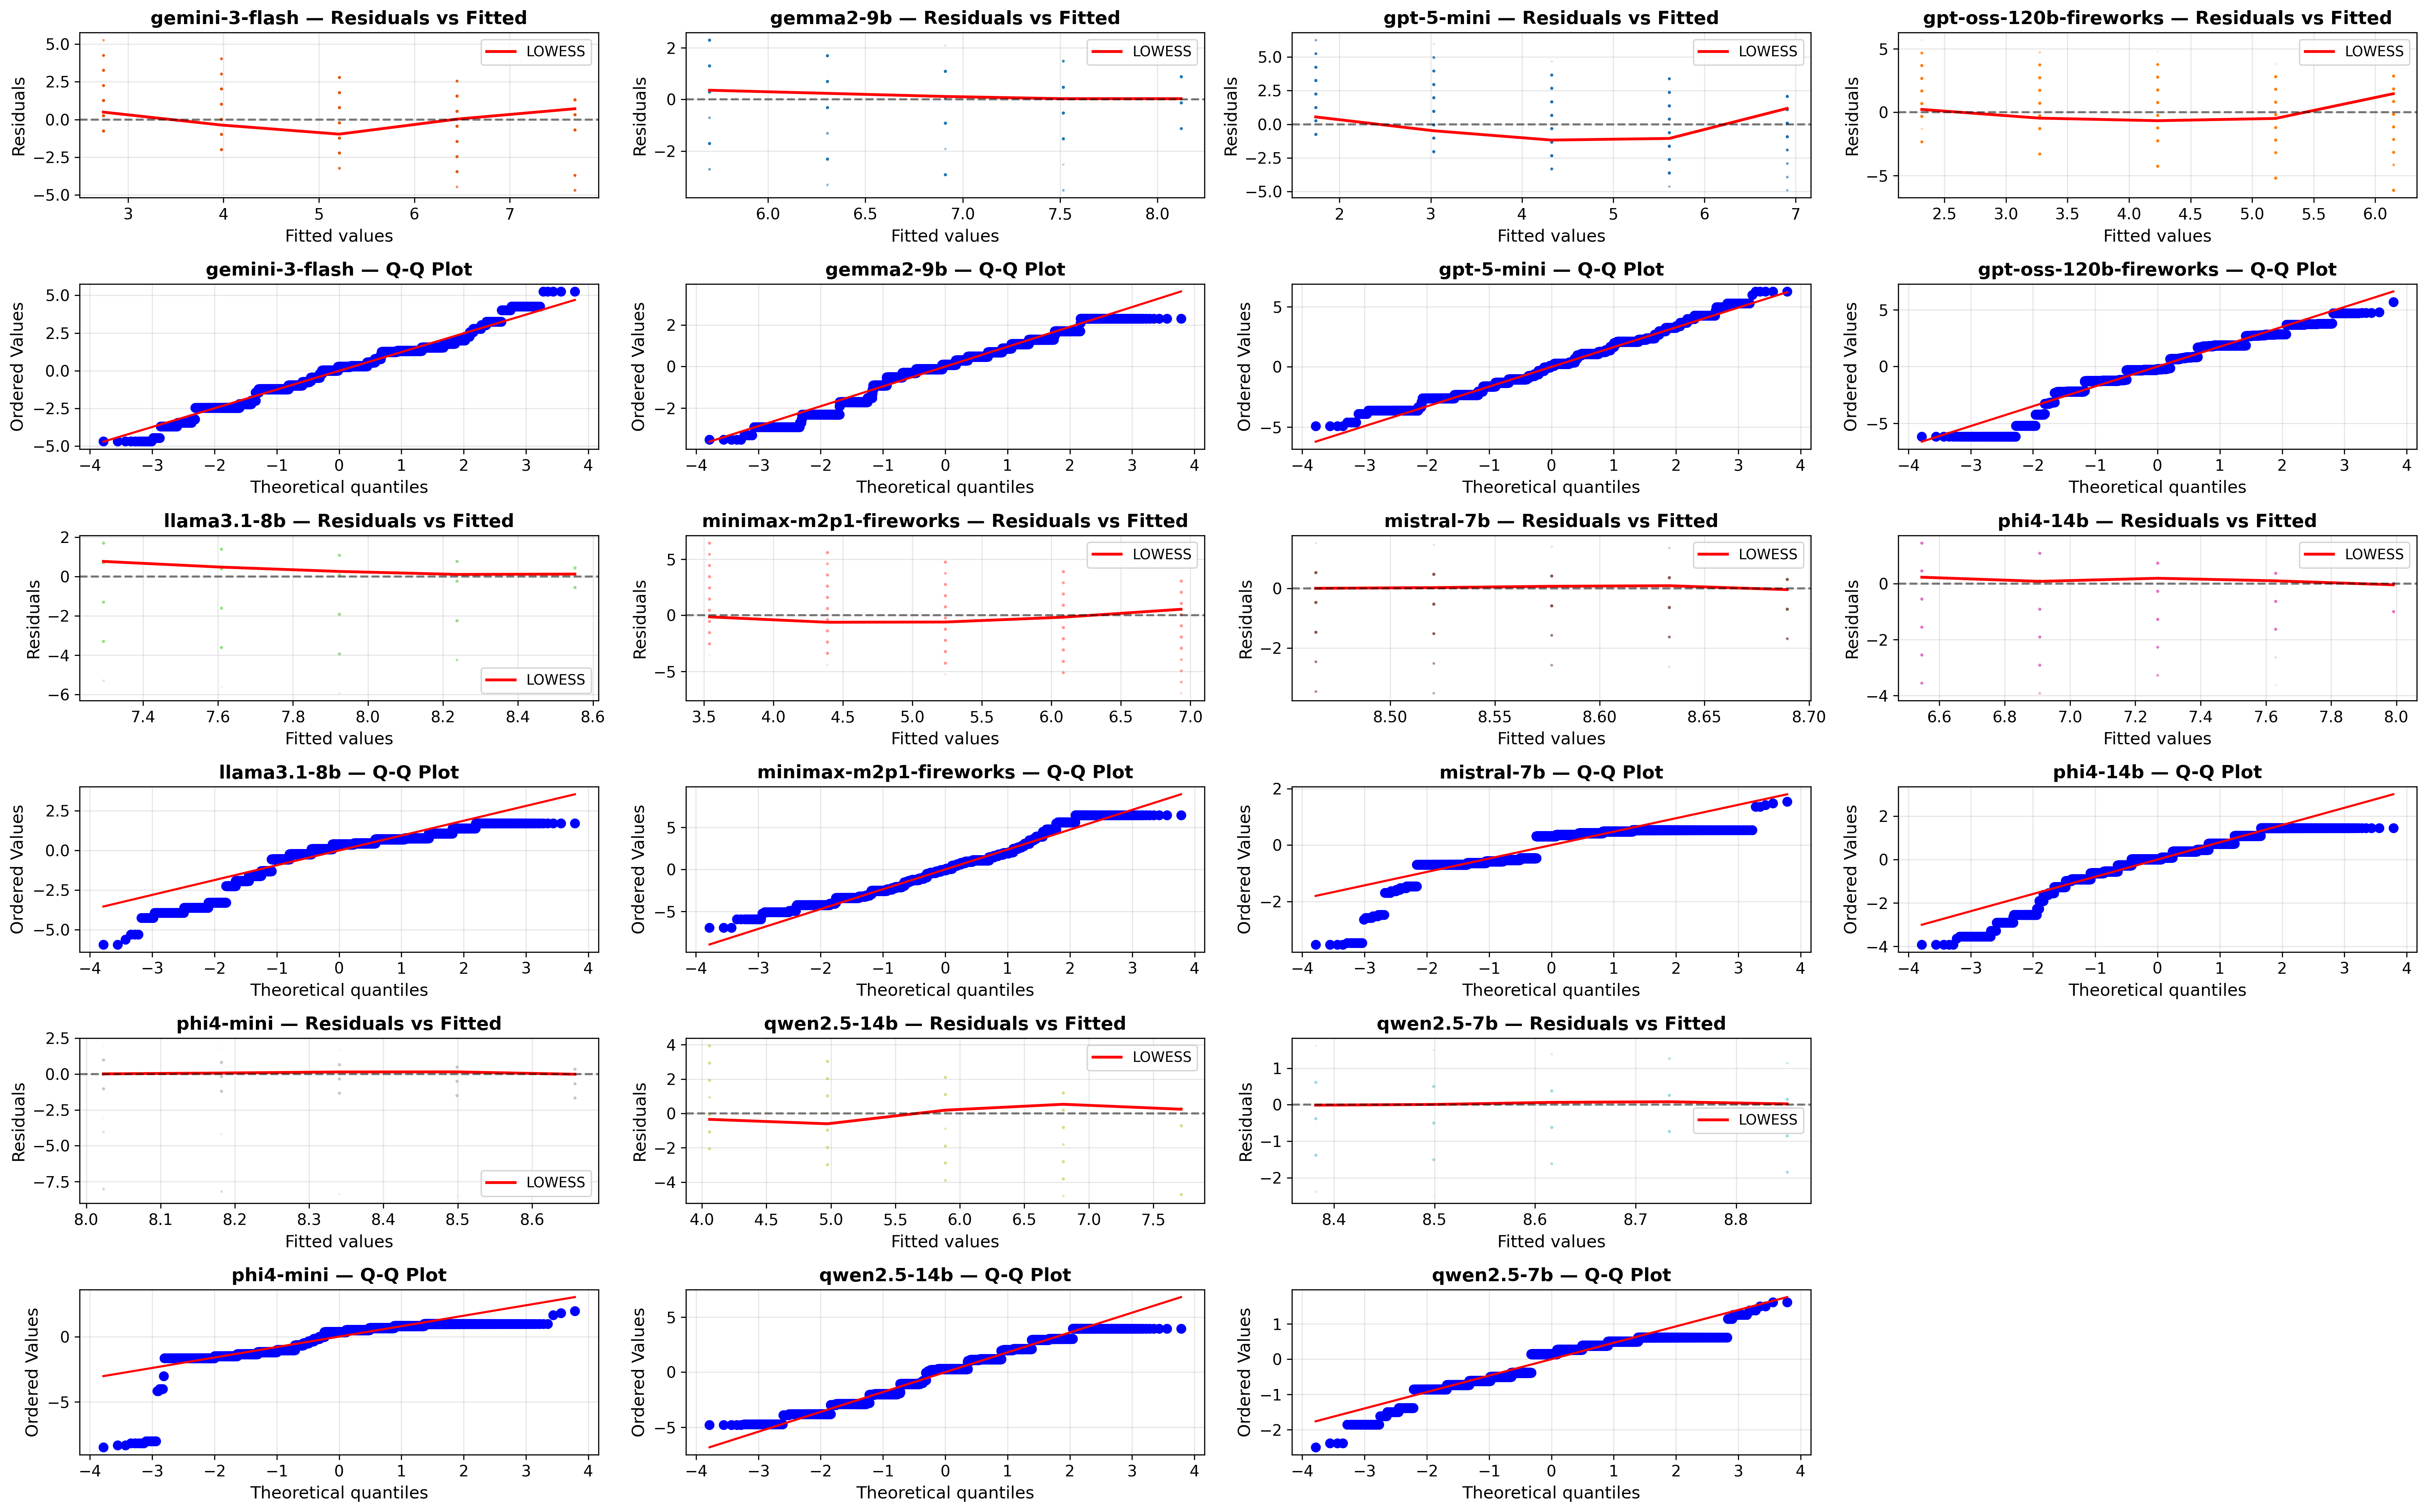
\includegraphics[width=\linewidth,height=0.85\textheight,keepaspectratio]{G14_residuals.png}
\caption{Residual diagnostics from linear regression. Left: residuals
vs.\ fitted with LOWESS smoother, showing systematic curvature. Right:
Q-Q plots showing heavy-tailed discrete residuals.}
\label{fig:residuals}
\end{figure}

\begin{figure}[htbp]
\centering
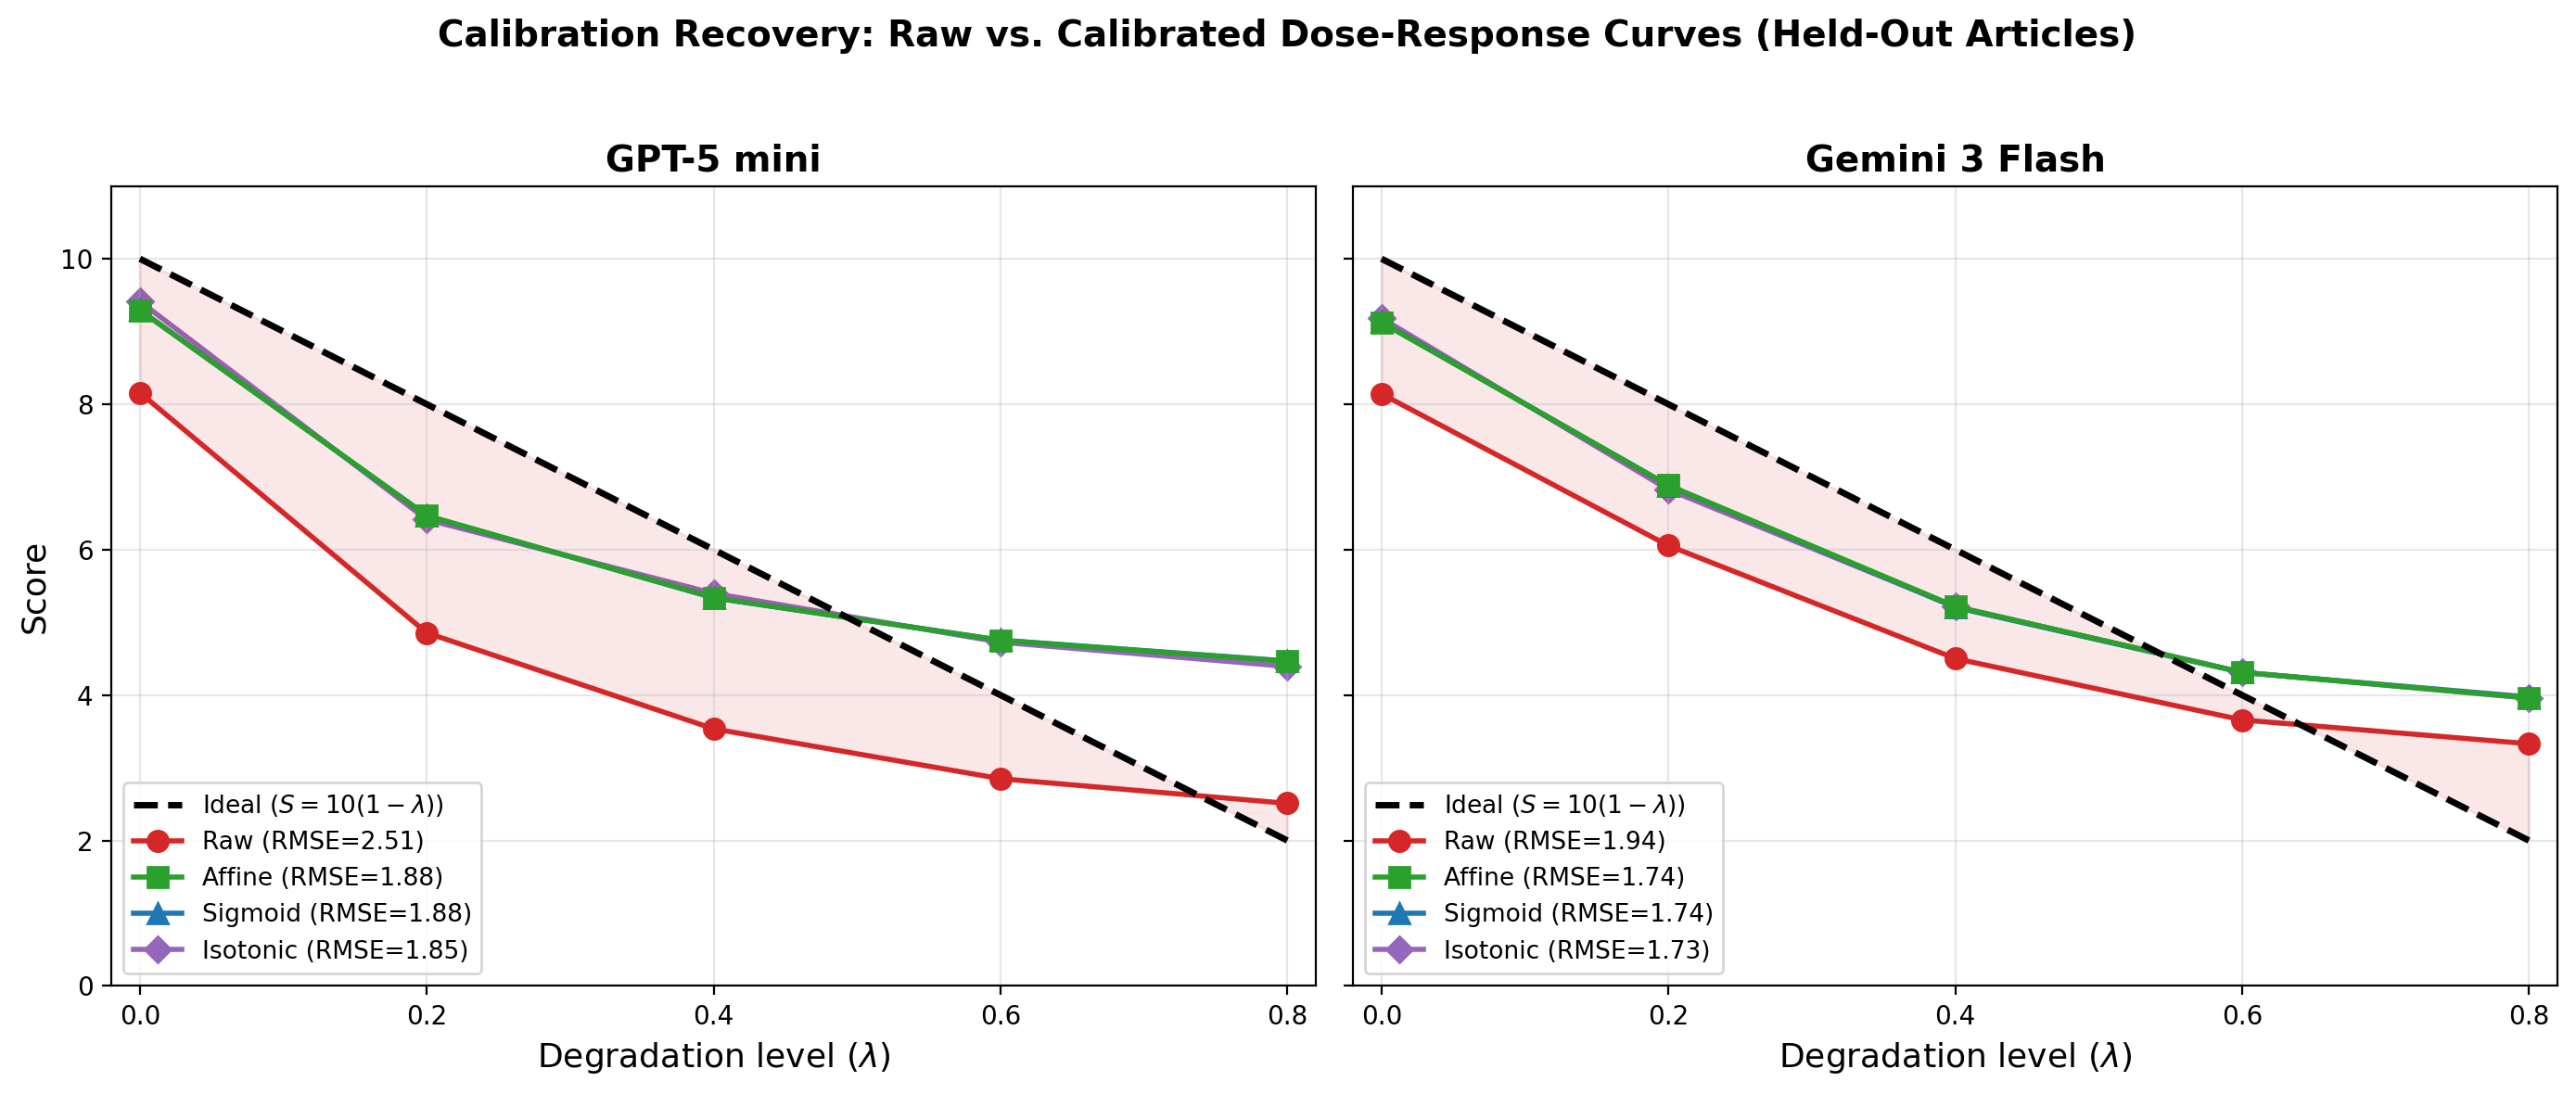
\includegraphics[width=\linewidth]{G15_calibration_recovery.png}
\caption{Dose-response curves before and after calibration. Affine,
sigmoid, and isotonic calibrations converge to nearly identical curves;
residual error is irreducible rank-order noise.}
\label{fig:calibrecovery}
\end{figure}

\begin{figure}[htbp]
\centering
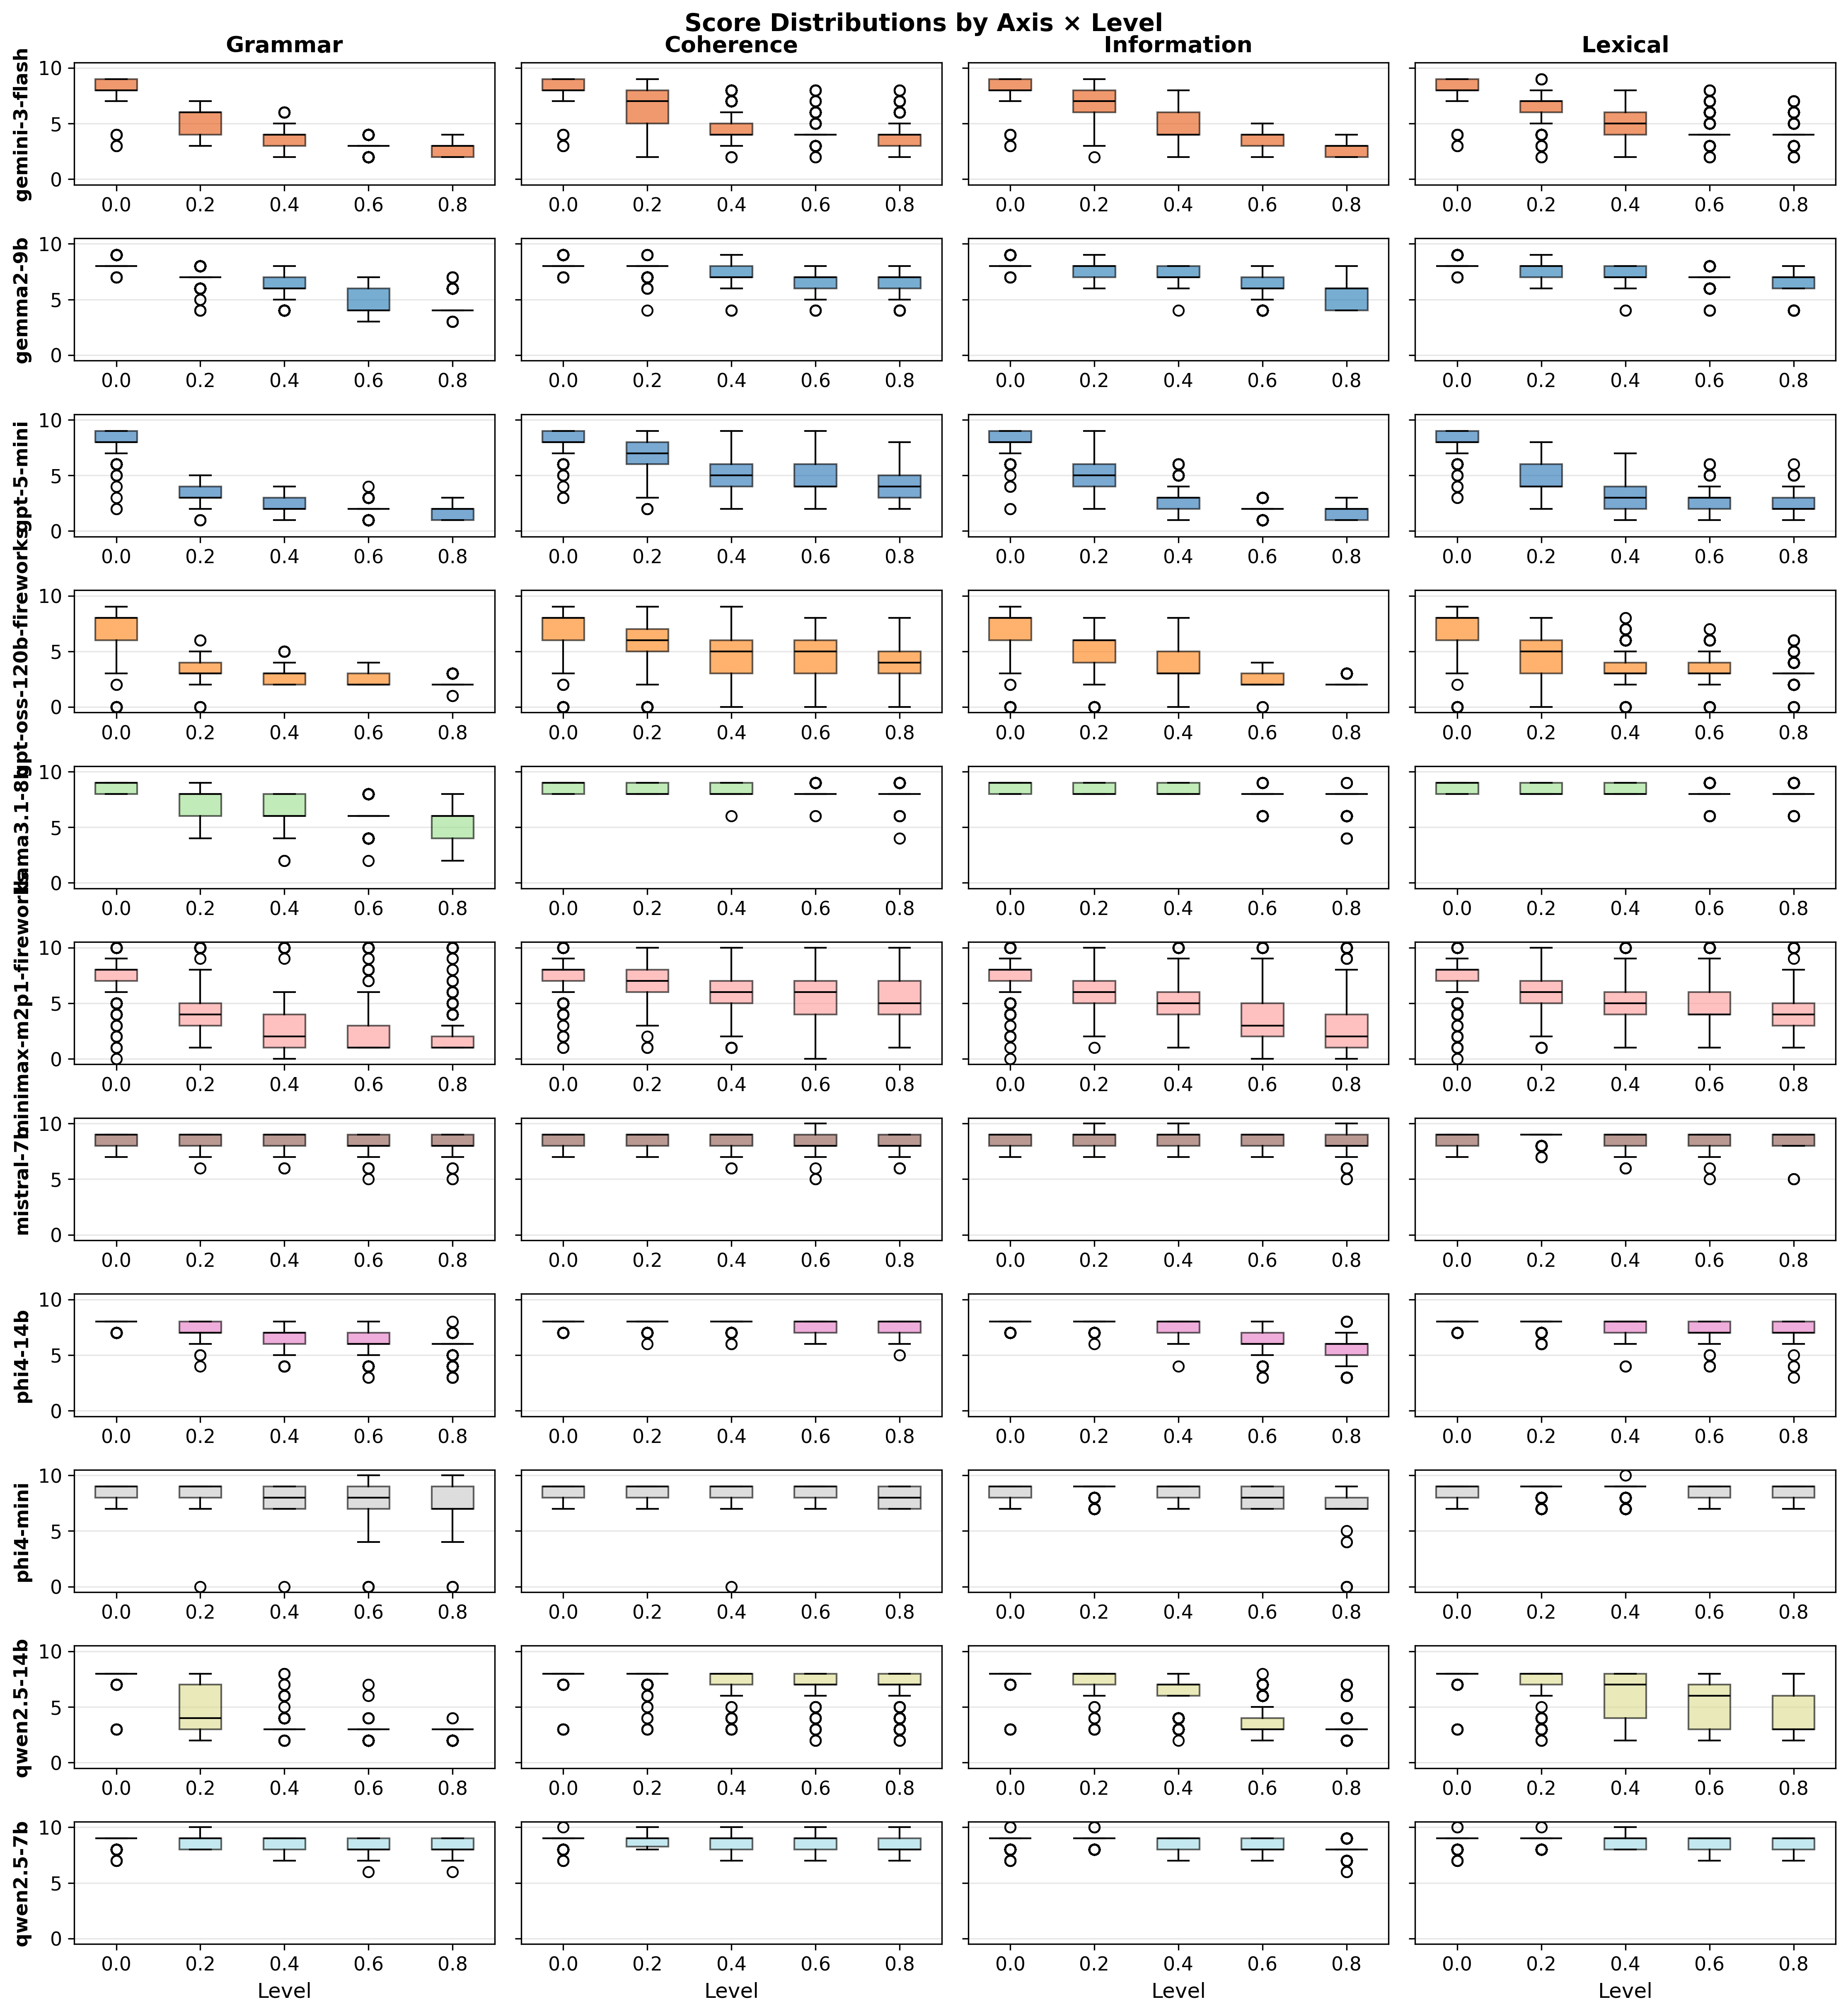
\includegraphics[width=\linewidth,keepaspectratio]{G6_boxplots_grid.png}
\caption{Score distributions by axis and level. IQR is narrowest at
highest and lowest degradation levels, reflecting ceiling and floor
compression.}
\label{fig:boxplots}
\end{figure}

\begin{figure}[htbp]
\centering
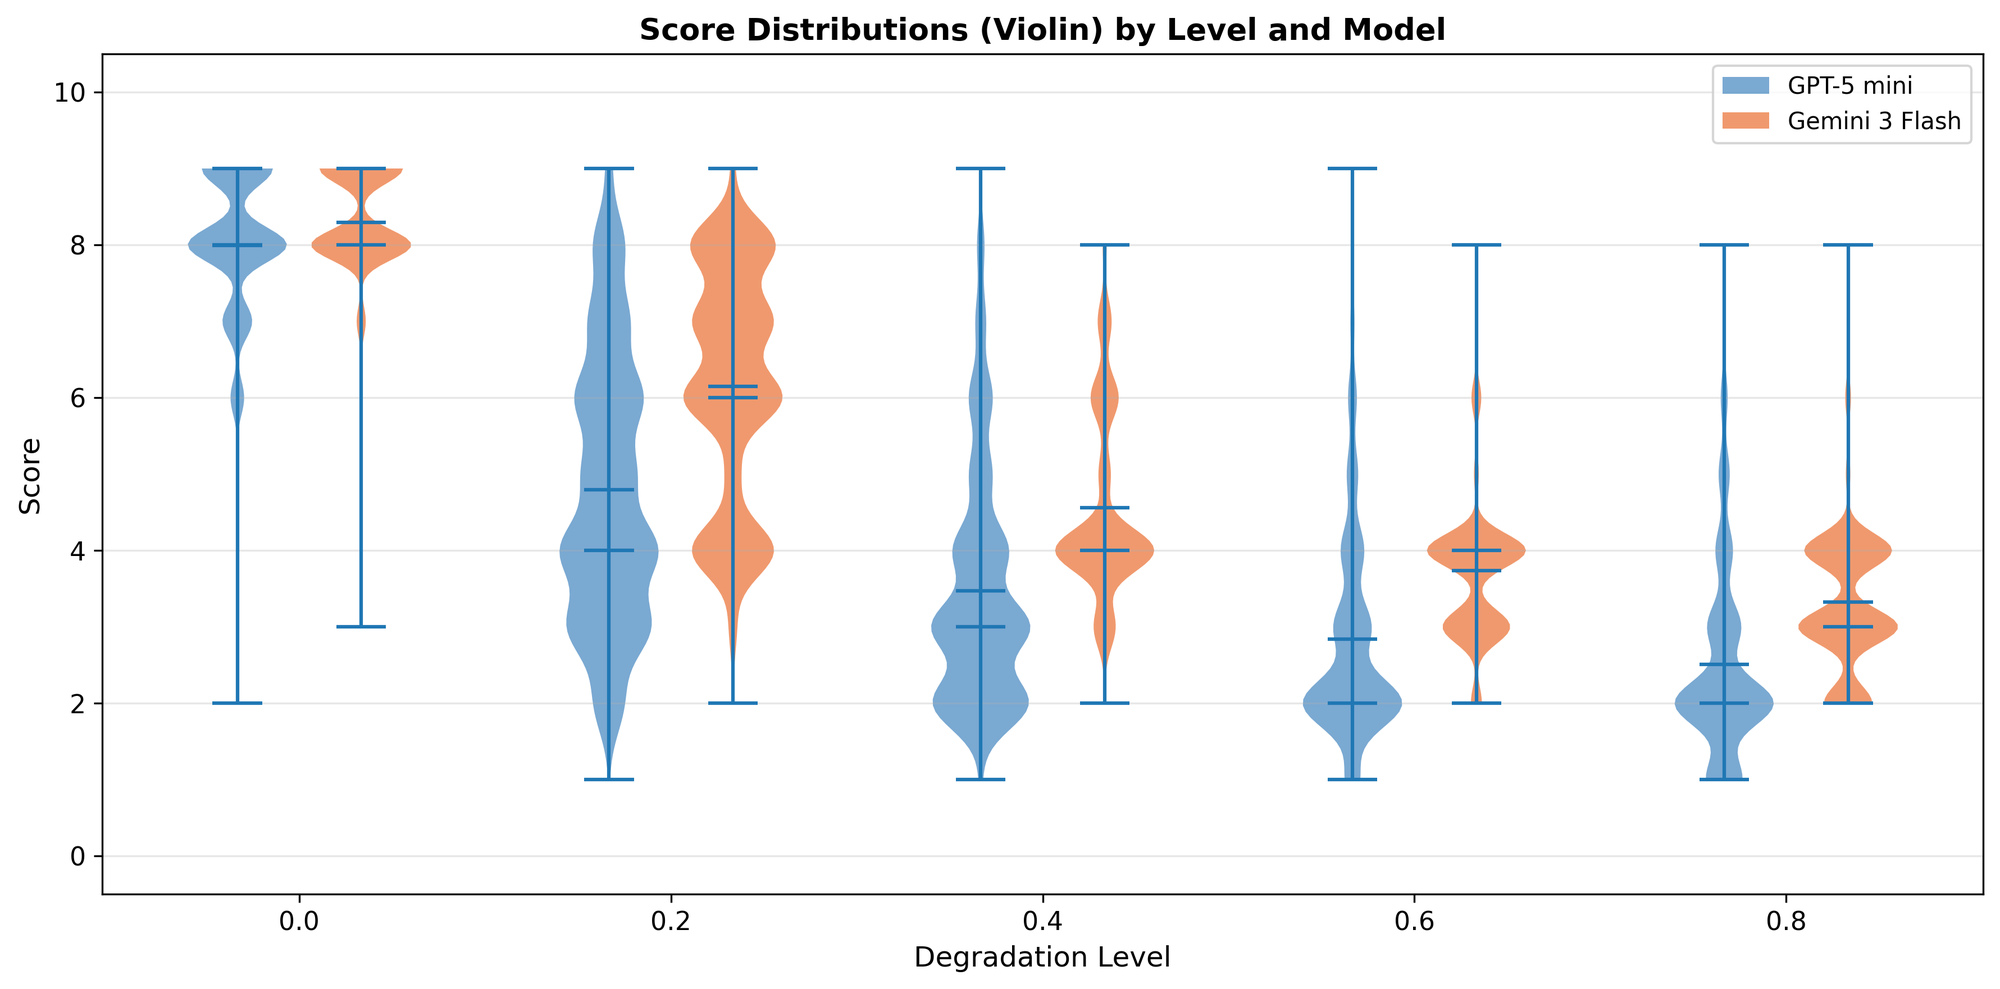
\includegraphics[width=\linewidth,keepaspectratio]{G7_violins.png}
\caption{Violin plots by degradation level and model. Bimodal shape at
$\lambda = 0.2$ reflects the onset of degradation effects.}
\label{fig:violins}
\end{figure}

\end{document}